% Options for packages loaded elsewhere
\PassOptionsToPackage{unicode}{hyperref}
\PassOptionsToPackage{hyphens}{url}
\PassOptionsToPackage{dvipsnames,svgnames*,x11names*}{xcolor}
%
\documentclass[
  11pt,
]{article}
\usepackage[]{mathpazo}
\usepackage{amsmath}
\usepackage{ifxetex,ifluatex}
\ifnum 0\ifxetex 1\fi\ifluatex 1\fi=0 % if pdftex
  \usepackage[T1]{fontenc}
  \usepackage[utf8]{inputenc}
  \usepackage{textcomp} % provide euro and other symbols
  \usepackage{amssymb}
\else % if luatex or xetex
  \usepackage{unicode-math}
  \defaultfontfeatures{Scale=MatchLowercase}
  \defaultfontfeatures[\rmfamily]{Ligatures=TeX,Scale=1}
\fi
% Use upquote if available, for straight quotes in verbatim environments
\IfFileExists{upquote.sty}{\usepackage{upquote}}{}
\IfFileExists{microtype.sty}{% use microtype if available
  \usepackage[]{microtype}
  \UseMicrotypeSet[protrusion]{basicmath} % disable protrusion for tt fonts
}{}
\usepackage{xcolor}
\IfFileExists{xurl.sty}{\usepackage{xurl}}{} % add URL line breaks if available
\IfFileExists{bookmark.sty}{\usepackage{bookmark}}{\usepackage{hyperref}}
\hypersetup{
  pdftitle={Making Migration Sexy: How State and National Policies Influence International Migration of Same-Sex Couples},
  pdfauthor={Nathan I. Hoffmann, Department of Sociology, University of California, Los Angeles; Kristopher Velasco, Department of Sociology, Princeton University},
  pdfkeywords={immigration, same-sex couples, LGB policy, sexuality},
  colorlinks=true,
  linkcolor=blue,
  filecolor=Maroon,
  citecolor=Blue,
  urlcolor=Blue,
  pdfcreator={LaTeX via pandoc}}
\urlstyle{same} % disable monospaced font for URLs
\usepackage[margin=1in]{geometry}
\usepackage{longtable,booktabs}
\usepackage{calc} % for calculating minipage widths
% Correct order of tables after \paragraph or \subparagraph
\usepackage{etoolbox}
\makeatletter
\patchcmd\longtable{\par}{\if@noskipsec\mbox{}\fi\par}{}{}
\makeatother
% Allow footnotes in longtable head/foot
\IfFileExists{footnotehyper.sty}{\usepackage{footnotehyper}}{\usepackage{footnote}}
\makesavenoteenv{longtable}
\usepackage{graphicx}
\makeatletter
\def\maxwidth{\ifdim\Gin@nat@width>\linewidth\linewidth\else\Gin@nat@width\fi}
\def\maxheight{\ifdim\Gin@nat@height>\textheight\textheight\else\Gin@nat@height\fi}
\makeatother
% Scale images if necessary, so that they will not overflow the page
% margins by default, and it is still possible to overwrite the defaults
% using explicit options in \includegraphics[width, height, ...]{}
\setkeys{Gin}{width=\maxwidth,height=\maxheight,keepaspectratio}
% Set default figure placement to htbp
\makeatletter
\def\fps@figure{htbp}
\makeatother
\setlength{\emergencystretch}{3em} % prevent overfull lines
\providecommand{\tightlist}{%
  \setlength{\itemsep}{0pt}\setlength{\parskip}{0pt}}
\setcounter{secnumdepth}{5}
\usepackage{fancyhdr}
\pagestyle{fancy}
\setlength{\headheight}{13.6pt}
\rhead{\textit{Hoffmann and Velasco}}
\lhead{\textit{August 25, 2021}}
\usepackage{booktabs}
\usepackage{longtable}
\usepackage{array}
\usepackage{multirow}
\usepackage{wrapfig}
\usepackage{float}
\usepackage{colortbl}
\usepackage{pdflscape}
\usepackage{tabu}
\usepackage{threeparttable}
\usepackage{threeparttablex}
\usepackage[normalem]{ulem}
\usepackage{makecell}
\usepackage{xcolor}
\ifluatex
  \usepackage{selnolig}  % disable illegal ligatures
\fi
\newlength{\cslhangindent}
\setlength{\cslhangindent}{1.5em}
\newlength{\csllabelwidth}
\setlength{\csllabelwidth}{3em}
\newenvironment{CSLReferences}[2] % #1 hanging-ident, #2 entry spacing
 {% don't indent paragraphs
  \setlength{\parindent}{0pt}
  % turn on hanging indent if param 1 is 1
  \ifodd #1 \everypar{\setlength{\hangindent}{\cslhangindent}}\ignorespaces\fi
  % set entry spacing
  \ifnum #2 > 0
  \setlength{\parskip}{#2\baselineskip}
  \fi
 }%
 {}
\usepackage{calc}
\newcommand{\CSLBlock}[1]{#1\hfill\break}
\newcommand{\CSLLeftMargin}[1]{\parbox[t]{\csllabelwidth}{#1}}
\newcommand{\CSLRightInline}[1]{\parbox[t]{\linewidth - \csllabelwidth}{#1}\break}
\newcommand{\CSLIndent}[1]{\hspace{\cslhangindent}#1}

\title{Making Migration Sexy: How State and National Policies Influence International Migration of Same-Sex Couples\thanks{The authors contributed equally to this paper. We thank Roger Waldinger, Margaret Peters, Filiz Garip, the Migration Working Group at UCLA, and participants at the Annual Meetings of the American Sociological Association and the Population Association of America for their helpful feedback.}}
\author{Nathan I. Hoffmann, Department of Sociology, University of California, Los Angeles \and Kristopher Velasco, Department of Sociology, Princeton University}
\date{August 25, 2021}

\begin{document}
\maketitle
\begin{abstract}
Both internationally and in the U.S., the policy landscape for same-sex couples is changing rapidly. Yet few researchers have studied the relationship between LGB rights and immigration on a large scale, even as surveys report rapidly increasing numbers of immigrant same-sex couples in the U.S. Using the American Community Survey from 2008 to 2019 and original datasets indexing LGB policy changes in 193 countries and all U.S. states over 29 years, this study characterizes and assesses the scale of LGB migration to the U.S. as well as the role of LGB policy. Compared to different-sex immigrant couples, immigrants in same-sex couples come from richer, more democratic countries that are less represented in immigrant networks. Contrary to previous work focusing on LGB immigrants from repressive contexts, fixed effects models show that these immigrants are more likely to come from LGB-friendly countries. They are also more likely to live in progressive U.S. states, an effect that increases in strength as migrants come from more LGB-friendly countries of origin. These findings highlight how sexuality as well as state policies seemingly unrelated to migration can shape aspirations and capabilities to migrate.
\end{abstract}

\hypertarget{introduction}{%
\section{Introduction}\label{introduction}}

In 2013, the U.S. Supreme Court overturned the Defense of Marriage Act and required the U.S. government to begin recognizing marriages between same-sex spouses. Among many consequences, this decision radically changed the immigration landscape: For the first time, same-sex spouses of U.S. citizens and legal permanent residents were eligible to file a spousal petition for an immigrant visa (\protect\hyperlink{ref-edwards_2013}{Edwards, 2013}). In the years since, the U.S. population of immigrants in same-sex couples has grown rapidly. While numbers of different-sex couples including immigrants increased by 13 percent from 2013 to 2019 (from 8.4 million to 9.5 million), those of corresponding same-sex couples grew from 61 thousand to 107 thousand in the same period, an increase of 76 percent. While some descriptions of this burgeoning population exist (\protect\hyperlink{ref-gates_2013}{Gates, 2013a}; \protect\hyperlink{ref-goldberg_2021}{Goldberg \& Conron, 2021}), there is a pressing need to understand the forces influencing their migration into the U.S.

The Supreme Court ruling occurred against a backdrop of rapidly changing laws concerning same-sex couples -- and LGB communities, generally -- both in the U.S. and abroad. As some countries expanded rights and social recognition, others imposed new forms of repression (\protect\hyperlink{ref-hadler_2018_world}{Hadler \& Symons, 2018}). These varied dynamics raise an important question: How do changing policy environments influence the migration patterns of individuals in same-sex couples into and across the U.S.? While gender is increasingly recognized as an integral part of the migration process (\protect\hyperlink{ref-hondagneu-sotelo_2012}{Hondagneu-Sotelo, 2012}; \protect\hyperlink{ref-lutz_2010}{Lutz, 2010}), sexuality receives relatively scant attention. Moreover, migration scholarship is only recently recognizing the role of the state to shape both the aspirations and capabilities to migrate through social policies, even those unrelated to migration itself (\protect\hyperlink{ref-dehaas_2021}{de Haas, 2021}; \protect\hyperlink{ref-fitzgerald_2014}{Fitzgerald et al., 2014}). Emerging qualitative work has demonstrated, however, that both sexuality and the policies governing it are highly salient factors influencing migration decisions to the U.S. (\protect\hyperlink{ref-ahmad_2013}{Ahmad, 2013}; \protect\hyperlink{ref-carrillo_2018}{Carrillo, 2018}; \protect\hyperlink{ref-gorman-murray_2009}{Gorman-Murray, 2009}; \protect\hyperlink{ref-mai_2009}{Mai \& King, 2009}). Studying the migration of same-sex couples into and across the U.S. allows us to make broader inferences into how the interaction between sexuality and policy shape migration decisions, underscoring the importance of political and ``lifestyle'' considerations into understandings of migration (\protect\hyperlink{ref-benson_2012}{Benson \& O'Reilly, 2012}; \protect\hyperlink{ref-fitzgerald_2014}{Fitzgerald et al., 2014}).

To address our research question, we evaluate how LGB policies at country of origin and U.S. state of residence relate to the migratory patterns for immigrants cohabiting with a same-sex partner. We do so by integrating two types of data. First, we rely on American Community Survey (ACS) data from 2008 to 2019 (\protect\hyperlink{ref-ruggles_2021}{Ruggles et al., 2021}), which allows the identification of individuals in cohabiting same-sex couples as well as their country of origin, U.S. state of residence, and potentially confounding individual characteristics. Second, we harness original datasets indexing LGB policy changes in 193 countries and all U.S. states from 1991 to 2019 (\protect\hyperlink{ref-velasco_2020}{Velasco, 2020}). We merge these two primary data sources with country- and state-level control variables from the UN, World Bank, U.S. government, and other sources.

Our analytic strategy proceeds in four parts. First, we descriptively understand who these cohabiting LGB immigrants are. This first step is important because little is known about this growing population. Second, we focus on country-of-origin effects, modeling how representation of immigrants in same-sex partnerships changes over time in relation to the LGB policy context of the country of origin. Third, we factor in the role of changing state LGB policy context in models at the U.S. state level. Lastly, we shift our attention to the individual, assessing how being an immigrant in a same-sex couple, net of other individual factors, bears upon choice of LGB policy context by state. We also consider how this relationship is moderated by LGB policy context in the country of origin.

Our investigation finds that origin countries with more LGB-friendly policies send higher proportions of immigrants in same-sex couples into the U.S., offering an important intervention into queer migration studies. In line with the aspirations-capabilities framework (\protect\hyperlink{ref-dehaas_2021}{de Haas, 2021}), affirming policies enable the migration projects of LGB individuals and provide the necessary material and symbolic resources, whereas oppressive policies hinder such ambitions. This finding is unexpected given existing queer migration scholarship which largely focuses on asylum seekers seeking entry into the U.S. and western countries, generally, from repressive origin-country contexts. Our findings also indicate that immigrants in same-sex couples are more likely to reside in U.S. states with progressive policies, especially as they come from countries with more supportive policies as well. By showing how policies seemingly unrelated to migration can shape migration decisions and actions, this projects shows how identity -- and the state's governance of it -- can interact with broader institutional contexts to yield unexpected results.

\hypertarget{background-changing-policy-landscape-for-same-sex-immigrant-couples}{%
\section{Background: Changing Policy Landscape for Same-Sex Immigrant Couples}\label{background-changing-policy-landscape-for-same-sex-immigrant-couples}}

The U.S. continues to undergo significant shifts in the policies governing LGB populations at both state and federal levels. Since 2003, the U.S. Supreme Court has ruled sodomy laws and the Defense of Marriage Act unconstitutional, recognized same-sex marriages at the federal level, and curtailed employment discrimination. In response, though, several U.S. states implemented new policies hindering LGB communities on top of existing discriminatory practices like state constitutional bans on marriage equality (\protect\hyperlink{ref-kazyak_2018}{Kazyak et al., 2018}). These dynamics create a varied landscape in which state lines significantly demarcate the types of rights and legal environments LGB people experience. Now, a burgeoning area of scholarship exists to understand the causes of these transformations (\protect\hyperlink{ref-lax_2009}{Lax \& Phillips, 2009}; \protect\hyperlink{ref-soule_2004}{Soule, 2004}) and their distinct consequences on the lives and well-being of LGB people (\protect\hyperlink{ref-boertien_2019}{Boertien \& Vignoli, 2019}; \protect\hyperlink{ref-carpenter_2020}{Carpenter, 2020}; \protect\hyperlink{ref-kail_2015}{Kail et al., 2015}; \protect\hyperlink{ref-levy_2017}{Levy \& Levy, 2017}).

Although this changing policy landscape affects LGB populations of all types, particular sub-groups within this broad umbrella are differentially impacted. Same-sex immigrant couples represent a population especially vulnerable to recent changes. This is because prior to being able to experience recognized rights like marriage or non-discrimination protections, immigrants in same-sex couples must first be able to enter into the U.S. Historically, federal U.S. law hindered such couples' ability to enter the country due to the government's lack of recognition of their relationship (\protect\hyperlink{ref-humanrightswatch_2006}{Human Rights Watch, 2006}). One of the few mechanisms available to queer migrants for entering the U.S. was through asylum claims -- an invasive process requiring migrants to ``prove'' their sexual desires and potential persecution (\protect\hyperlink{ref-humanrightswatch_2006}{Human Rights Watch, 2006}).

These broad legal exclusions often carry over to academic scholarship as well. Analyses of domestic LGB communities often assume citizenship and migration research presents migrants as heterosexual (\protect\hyperlink{ref-luibheid_2008}{Luibhéid, 2008}). The academic research that does acknowledge the realities of queer migrants, though, is largely centered on the asylum claims and offers qualitative insights into how queer migrants navigate this process (\protect\hyperlink{ref-vogler_2016}{Vogler, 2016}). As such, there is presently a shallow understanding of the factors broadly influencing the migratory patterns of same-sex immigrant couples beyond this pathway and how these patterns align or diverge from their well-studied heterosexual counterparts.
This omission is especially stark considering that those migrating for family-related reasons, such as this, historically outnumber those migrating for other reasons, even work (\protect\hyperlink{ref-kandel_2018_familybased}{Kandel} (\protect\hyperlink{ref-kandel_2018_familybased}{2018})).

\begin{figure}
\centering
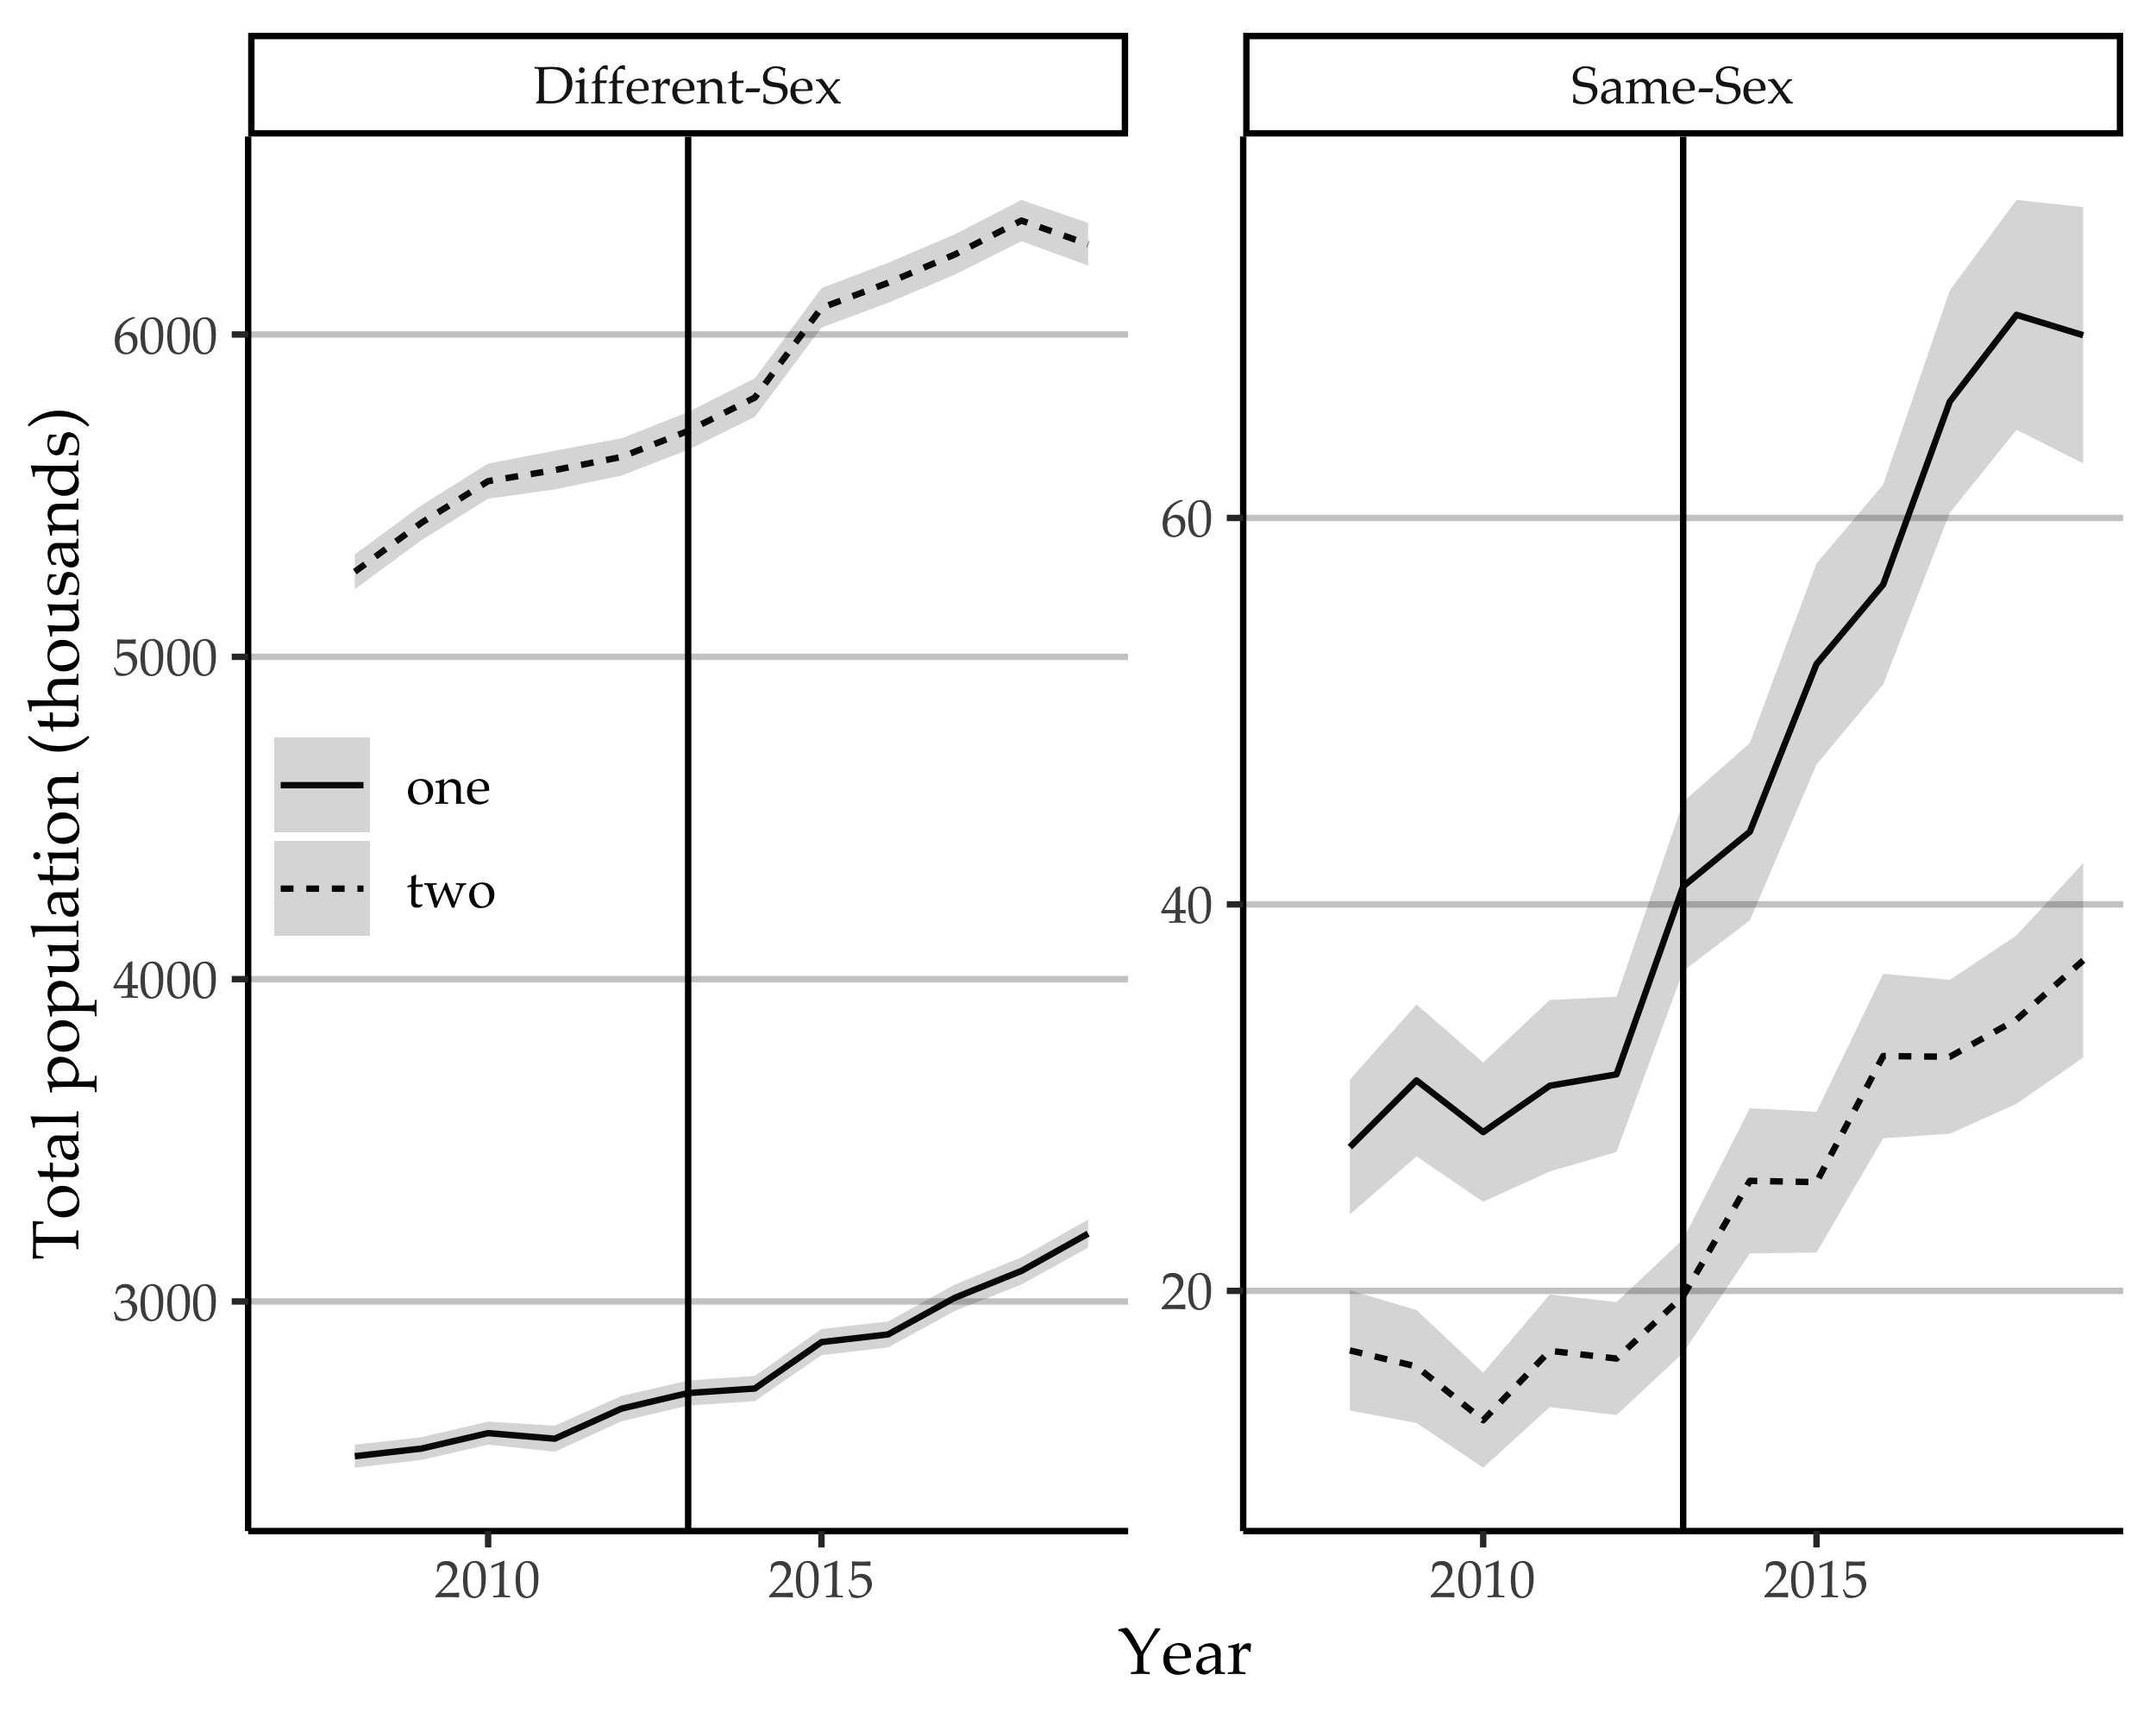
\includegraphics{ssimm_draft_files/figure-latex/total-pop-1.pdf}
\caption{\label{fig:total-pop}Estimated totals of different- and same-sex couples containing one or two immigrants, 2008-2019, with 95\% confidence intervals. Vertical line placed at the year 2013, when DOMA was overturned.}
\end{figure}

The federal environment governing immigration significantly changed after 2013. The U.S. Supreme Court opinion ruling the Defense of Marriage Act (DOMA) unconstitutional opened the door for more same-sex immigrant couples to enter the U.S. under the same process long-governing different-sex couples (\protect\hyperlink{ref-edwards_2013}{Edwards, 2013}). Indeed, as Figure \ref{fig:total-pop} highlights, the number of same-sex immigrant couples in the U.S. grew significantly following this ruling -- especially when compared to different-sex couples. Aside from allowing gay and lesbian families to remain unified, this national opening creates an important moment for the scholarly community as well. Now, more careful investigations into the factors enabling and constraining the movement of same-sex immigrant couples into the U.S. can be conducted beyond idiosyncratic asylum claims. The present research fits squarely within this critical research gap.

\hypertarget{understanding-influences-on-migration-patterns}{%
\section{Understanding Influences on Migration Patterns}\label{understanding-influences-on-migration-patterns}}

\hypertarget{conventional-explanations}{%
\subsection{Conventional Explanations}\label{conventional-explanations}}

Our analysis compares conventional explanations for migration to political ones related to LGB policy. Massey et al. (\protect\hyperlink{ref-massey_1999}{1999, p. 50}) provided an influential synthesis of migration theories from sociology, economics, and anthropology, arguing that ``causal processes relevant to international migration might operate on multiple levels simultaneously.'' Our investigation incorporates insights from their work as well as assesses how sexuality and LGB policy complicate migration research. At one level, neoclassical economic theories underscore that promise of material gain is a frequent motivation to migrate (\protect\hyperlink{ref-hatton_2005a}{Hatton \& Williamson, 2005}; \protect\hyperlink{ref-todaro_1980}{Todaro, 1980}), predicting that migrants will follow wage and unemployment differentials across countries. To account for migration costs, these models often adjust for distance: Immigrants are more likely to migrate between proximate countries, especially those that share a border. At another level, migration streams often continue in a process of cumulative causation even after wage differentials decrease (\protect\hyperlink{ref-massey_1990_social}{Massey, 1990}); this is due in large part to immigrant networks migrants that share information and resources to lower the cost of migration and settling in the destination country (\protect\hyperlink{ref-massey_1987}{Massey et al., 1987}) as well as institutions that arise to ease entry and settlement (\protect\hyperlink{ref-hernandez-leon_2013}{Hernández-León, 2013}). Quantitative scholars often measure immigration networks using the relative size of co-national immigrant stock (\protect\hyperlink{ref-beine_2016}{Beine et al., 2016}).

The theories synthesized by \protect\hyperlink{ref-massey_1999}{Massey et al.} (\protect\hyperlink{ref-massey_1999}{1999}) remained largely materialistic.
Our study heeds Garip's (\protect\hyperlink{ref-garip_2016}{2016}) call to explore migrant heterogeneity, assessing what the theories of migration synthesized by \protect\hyperlink{ref-massey_1999}{Massey et al.} (\protect\hyperlink{ref-massey_1999}{1999}) might miss when accounting for the migration of this LGB subpopulation. Recent research has shown that not only physical but cultural proximity can matter to the migration process; scholars have shown that shared language, colonial history, and democracy matter in the sending country (\protect\hyperlink{ref-karemera_2000}{Karemera et al., 2000}; \protect\hyperlink{ref-mayda_2010}{Mayda, 2010}), and immigrant rights matter in the receiving country (\protect\hyperlink{ref-fitzgerald_2014}{Fitzgerald et al., 2014}). Work on the relationship between welfare policies and immigration suggests that social policies not explicitly related to the latter can impact the migration and settlement processes. Historically, welfare and immigration were tightly linked in the U.S. (\protect\hyperlink{ref-fox_2012}{Fox, 2012}), and welfare generosity may play a role in shaping choice of destination for prospective emigrants today (\protect\hyperlink{ref-ferwerda_2021_pull}{Ferwerda \& Gest, 2021}; \protect\hyperlink{ref-razin_2015}{Razin \& Wahba, 2015}). Our research builds on these insights to test how non-welfare social policy specific to LGB individuals may influence their migration and settlement.

\hypertarget{sexuality-in-an-aspirations-capabilities-framework}{%
\subsection{Sexuality in an Aspirations-Capabilities Framework}\label{sexuality-in-an-aspirations-capabilities-framework}}

We incorporate the conventional migration theories discussed above into a broader aspirations-capabilities framework (\protect\hyperlink{ref-carling_2018_aspiration}{Carling \& Collins, 2018}; \protect\hyperlink{ref-dehaas_2021}{de Haas, 2021}; \protect\hyperlink{ref-schewel_2020}{Schewel, 2020}).
De Haas (\protect\hyperlink{ref-dehaas_2021}{2021, p. 17}) defines migration as ``a function of aspirations and capabilities to migrate within given sets of \emph{perceived} geographical opportunity structures'' (emphasis added). This framework blends individual, agentic motivations for migration (e.g., subjective desires and imaginations of well-being) with structural factors that condition these aspirations and the capabilities to act upon them (e.g., culture and policy). Thus, we use this framework to situation our intervention: to demonstrate why sexuality, and the state's governance of it, meaningfully contributes toward understandings of migration (\protect\hyperlink{ref-cantu_2009}{Cantú, 2009}; \protect\hyperlink{ref-carrillo_2018}{Carrillo, 2018}; \protect\hyperlink{ref-suen_2021_sexual}{Suen, 2021}).

The state plays an important role setting structural conditions that influence migratory pathways. One direct route is by establishing law governing migration itself. Indeed, significant scholarship details how such laws and policies are used to target distinct populations -- whether based on labor market needs (\protect\hyperlink{ref-castles_2006}{Castles, 2006}; \protect\hyperlink{ref-hahamovitch_2014}{Hahamovitch, 2014}), assistance following local disaster (\protect\hyperlink{ref-bekaert_2020}{Bekaert et al., 2020}; \protect\hyperlink{ref-hunter_2015}{Hunter et al., 2015}), or familial ties (\protect\hyperlink{ref-kofman_2004_family}{Kofman, 2004}). However, \protect\hyperlink{ref-dehaas_2021}{de Haas} (\protect\hyperlink{ref-dehaas_2021}{2021}) offers a more expansive view of the state. He contends that the state influences migration through policy that shapes individual's life aspirations and well-being -- whether real or imagined -- and by conditioning the capacity to migrate based on Berlin's (\protect\hyperlink{ref-berlin_1969_four}{1969}) negative and positive ``liberties.'' For example, explicit migration policy represents a ``negative liberty,'' whereby the state externally imposes opportunities and constraints, but liberal telecommunications policy that allows for the transnational flow of news, media, and information is a ``positive liberty'' that influences the capacity to migrate -- in this case by increasing knowledge of alternatives and the ``capacity to aspire'' (\protect\hyperlink{ref-dehaas_2021}{de Haas, 2021}). Therefore, the aspirations-capabilities framework is not a rejection of previous theories of migration, but a more expansive framework that acknowledges the subjective role of individuals to determine if migration advances their well-being within given conditions.

Sexuality has long factored into migratory decisions. However, as the global awareness of LGB rights expands, sexuality is increasingly an important factor shaping the aspirations and capabilities to leave one's home country (\protect\hyperlink{ref-mole_2018a}{Mole, 2018}; \protect\hyperlink{ref-murray_2016}{Murray, 2016}). This is partly due to international organizations' construction of sexuality as a legitimate basis for leaving. For example, in 2008 the United Nations High Commissioner for Refugees issued a new guidance note for why and how countries should consider sexual orientation and gender identity when granting asylum claims (\protect\hyperlink{ref-unhcr_2008}{UNHCR, 2008}). The note continues to guide various authorities to consider discriminatory domestic policies when evaluating asylum claims as such policies ``can create or contribute to an oppressive atmosphere of intolerance and generate a threat of prosecution'' (\protect\hyperlink{ref-unhcr_2008}{UNHCR, 2008, p. 8}). International organizations such as the European Union and several countries now incorporate this guidance (\protect\hyperlink{ref-giametta_2020}{Giametta, 2020}).

Therefore, the globalization of LGB rights -- along with the transnational flow of information, cultural content, general visibility, and changing policy environments that accompany it (\protect\hyperlink{ref-ayoub_2016}{Ayoub, 2016}; \protect\hyperlink{ref-ayoub_2017}{Ayoub \& Garretson, 2017}) -- are likely to influence the migration of LGB communities by changing aspirations and capabilities to migrate. Current research on the types of policy environments likely to influence the migration of those in same-sex couples, however, is both limited in scope and mixed in outcomes. Although family-related migration has long overshadowed work-related among permanent migrants to the U.S. (\protect\hyperlink{ref-kandel_2018_familybased}{Kandel, 2018}), theorization on the former has largely ignored same-sex couples (e.g. \protect\hyperlink{ref-kofman_2004_family}{Kofman, 2004}). Additionally, emerging scholarship at the intersection of sexuality and migration is overwhelmingly qualitative, preventing generalizations about this population.
Thus a broader portrait for how policy environments influence queer migration is urgently needed.

\hypertarget{how-policies-at-country-of-origin-influence-migration}{%
\subsection{How Policies at Country of Origin Influence Migration}\label{how-policies-at-country-of-origin-influence-migration}}

Much queer migration research suggests that migrants in same-sex relationships are largely escaping repressive contexts. Since U.S. policy environment did not define same-sex partners as ``family'' before 2013, asylum remained one of the few viable mechanisms for entry and dramatically limited the capacity to migrate into the U.S. (\protect\hyperlink{ref-luibheid_2008}{Luibhéid, 2008}; \protect\hyperlink{ref-vogler_2016}{Vogler, 2016}). Although the U.S. is less progressive and inviting compared to many other Western states, high-profile developments such as marriage equality can contribute to an imagined openness relative to many locations around the world. For example, access to gay content in film and on the Internet contributed toward Iranian refugees to seek sexual freedom in the West (\protect\hyperlink{ref-karimi_2020}{Karimi, 2020}). These asylum seekers assumed, or aspired to live in, more affirming environments and knew such countries allowed sexual orientation as a basis for asylum. Additionally, another strand of research documents people in more oppressive contexts seeking out partners in more equitable locations who can then sponsor them through the immigration process (\protect\hyperlink{ref-carrillo_2018}{Carrillo, 2018}; \protect\hyperlink{ref-corey-boulet_2019}{Corey-Boulet, 2019}). Consequently, as Adur (\protect\hyperlink{ref-adur_2018}{2018, p. 321}, emphasis theirs) summarizes, ``sexuality also shapes migration as LGBTI immigrants relocate in pursuit of spaces that they \emph{imagine} will be safer and more liberal.'' Though such studies suggest immigrants in same-sex couples are largely fleeing repressive contexts, to what extent is this representative of immigrants in same-sex couples more generally?

Alternatively, immigrants in same-sex couples may come from countries with greater recognition and access to sexuality-related rights and services. There are two interrelated reasons for this. First, affirming policy environments are likely to enable people's capacity to make such an important, expensive, move. Long-standing research on immigrant selection demonstrates that migrants are typically from stronger social positions -- more formal education, higher incomes, and more prestigious occupations (\protect\hyperlink{ref-feliciano_2020}{Feliciano, 2020}). Given the high barriers to migrating, supportive policies such as access to full marriage equality and protections against employment discrimination may enable the capacity to migrate by providing the necessary social, human, and economic capitals. Second, same-sex coupledom, like marriage, is a culturally contingent artifact (\protect\hyperlink{ref-philpot_2016_gay}{Philpot et al., 2016}). Consequently, the interactive dynamics between policy and culture within an immigrant's country of origin is likely to influence their desire to be part of a couple to begin with (\protect\hyperlink{ref-baiocco_2014_desire}{Baiocco et al., 2014}; \protect\hyperlink{ref-flores_2016_backlash}{Flores \& Barclay, 2016}; \protect\hyperlink{ref-ocobock_2020_leveraging}{Ocobock, 2020}; \protect\hyperlink{ref-suen_2021_sexual}{Suen, 2021}). Policies supportive of LGB communities normalize and validate such identities and partnerships (\protect\hyperlink{ref-ocobock_2020_leveraging}{Ocobock, 2020}) -- influencing those with same-sex attractions to imagine and aspire such possibilities for themselves. And, relatedly, being from a country where the state recognizes one's sexuality and validates these relationships may make survey respondents, once in the U.S., more comfortable disclosing such relationships. As such, immigrants from countries without this cultural and political background may be more reticent to desire or disclose same-sex partnership.

Scholarship on lifestyle migration supports these arguments. Benson and O'Reilly (\protect\hyperlink{ref-benson_2009}{2009, p. 608}) refer to lifestyle migration as the ``relocation of relatively affluent people within the developed world searching for a better way of life.'' Lifestyle migration is conceptualized as a highly individualized decision-making process as conceptualizations of ``better way of life'' differ drastically (\protect\hyperlink{ref-benson_2016}{Benson \& O'Reilly, 2016}). Supportive LGB policies may offer a structural opening by which same-sex couples have the opportunity and bandwidth to consider these individualistic choices.

\hypertarget{how-policies-at-u.s.-state-of-residence-influence-migration}{%
\subsection{How Policies at U.S. State of Residence Influence Migration}\label{how-policies-at-u.s.-state-of-residence-influence-migration}}

While these country-of-origin policies may enable the movement of same-sex couples out of their home country, the varied policy environments across U.S. states are likely to differentially encourage the entry of these couples. Though research often focuses on either country of origin or destination, part of our intervention is to study these in tandem to provide a more comprehensive understanding of migration (\protect\hyperlink{ref-fitzgerald_2008}{FitzGerald, 2008}; \protect\hyperlink{ref-luthra_2018}{Luthra et al., 2018}).

Typically, a strong predictor of where migrants locate within the U.S. are network effects -- they locate where their family, friends, and other social relations are located (\protect\hyperlink{ref-massey_1987}{Massey et al., 1987}; \protect\hyperlink{ref-palloni_2001}{Palloni et al., 2001}; \protect\hyperlink{ref-portes_1998}{Portes, 1998}). Existing research highlights that gay and lesbian couples within the U.S. were likely to leave states without marriage equality prior to national recognition (\protect\hyperlink{ref-beaudin_2017}{Beaudin, 2017}) and that queer migrants often have strong cross-national networks for relaying information (\protect\hyperlink{ref-stella_2020}{Stella \& Gawlewicz, 2020}). This likely results in a greater concentration of same-sex couples in states with marriage equality and other protective policies. Additionally, if migrants are coming from a country with greater legal protections, they are unlikely to want to relocate to a state where such rights are no longer recognized -- rendering the political environment acutely important. Of course, this is predicated on the assumption that migrants take such distinct sub-national variations into account -- which they very well may not. Consequently, the ``pull'' to individual states may operate independently from specific state laws affirming LGB people and their relationships.

Though limited, existing demographic research does give some insights into how immigrants in same-sex couples might choose their state of residence once in the U.S. Cohabiting same-sex couples already within the U.S. are more likely to reside in states in the Northeast and West, such as Vermont, Massachusetts, California, and Oregon (\protect\hyperlink{ref-gates_2013a}{Gates, 2013b}), that have often been at the forefront in safeguarding LGB rights. The same-sex population is growing most rapidly, however, in the Midwest and South (\emph{ibid.}). Regardless of state, same-sex couples are more concentrated in urban areas, although this is truer for men than women (\protect\hyperlink{ref-baumle_2009}{Baumle et al., 2009}). This evidence suggests that immigrants in same-sex couples are likely to choose progressive states and cities as their place of residence.

In sum, it is evident that sexuality and the policies governing it are salient factors driving migratory decisions -- either enabling the opportunity and flexibility for same-sex couples to make decisions that are best for them or by erecting an environment so repressive that it forces migrants to flee to where imagination of opportunity awaits. Despite qualitative examinations into queer migrants, especially asylum seekers, there is no large-\(N\) investigation into how significant transformation of LGB policies -- both globally and across U.S. states -- influence migration into the U.S. Therefore, this research seeks to fill this gap in the literature by providing such an analysis and to further understand how the changing policy landscapes are differentially influencing the lives of queer people depending on their social positions.

\hypertarget{data}{%
\section{Data}\label{data}}

\hypertarget{identifying-same-sex-couples-in-the-acs}{%
\subsection{Identifying Same-Sex Couples in the ACS}\label{identifying-same-sex-couples-in-the-acs}}

We merge individual-level data on immigrants in the U.S. with state- and country-level variables from a variety of datasets. The individual data come from the 2008 to 2019 ACS (\protect\hyperlink{ref-ruggles_2021}{Ruggles et al., 2021}). Each year, the ACS surveys a 1-percent representative sample of the U.S. population about their education, occupation, income, family structure, immigration status, country of origin, location, and a variety of other individual and household attributes. We define a same-sex couple as two individuals of the same sex in the same household who report their relationship as ``spouse'' or ``unmarried partner.'' We limit the sample to individuals who immigrated at the age of 18 or older and in 1991 or later.\footnote{The exception is for for Figure \ref{fig:total-pop}, where we include those who immigrated in any year, at age 18 or older.} Hence this analysis considers four types of couples: (1) two-immigrant couples who came to the U.S. together; (2) two-immigrant couples that formed once in the U.S.; (3) mixed status couples where an immigrant migrated to be with their U.S.-born partner; and (4) mixed status couples that formed in the U.S. As shown in the Supplementary Material, results do not differ substantively for one- or two-immigrant couples. We are unable to differentiate between couples that partnered or married abroad and those that do so in the U.S. We elaborate on the implications of these scope conditions in the Discussion.

The 12 years of survey data contain 6,349 same-sex couples that include at least one immigrant, for a total of 7,011 immigrants in same-sex couples with complete data. These immigrants are compared to 641,521 corresponding different-sex couples containing 898,869 individual immigrants. Below, we outline how we use these data to construct dependent variables based on each analysis. All analyses incorporate ACS sampling weights.

Measuring the prevalence of same-sex couples in the U.S. is difficult (\protect\hyperlink{ref-michaels_2013}{Michaels, 2013}). As in most nationally representative demographic work on same-sex couples (\protect\hyperlink{ref-baumle_2013}{Baumle, 2013}; \protect\hyperlink{ref-baumle_2019}{Baumle \& Dreon, 2019}), we are able to identify only LGB couples that cohabit; unpartnered LGB individuals and those who do not live with their partner are not included in the analysis (\protect\hyperlink{ref-baumle_2009}{Baumle et al., 2009, p. 6}). In addition, LGB individuals who do not feel comfortable with the partner labels of the ACS are not in the sample. Another pitfall is measurement error: Misreporting may result when different-sex couples accidentally misspecify the gender of one of the partners (\protect\hyperlink{ref-gates_2009}{Gates \& Steinberger, 2009}; \protect\hyperlink{ref-goodnature_2021}{Goodnature \& Neto, 2021}). Beginning in 2008 the Census Bureau made changes to ACS gender and partnership questions in order to prevent such errors (\protect\hyperlink{ref-u.s.censusbureau_2013}{U.S. Census Bureau, 2013}), so we rely on data only from 2008 onward, but difficulties remain. If even a small number of different-sex couples misreport one partner's sex, the counts of same-sex couples will be inflated. Following \protect\hyperlink{ref-gates_2009}{Gates \& Steinberger} (\protect\hyperlink{ref-gates_2009}{2009}), we remove all respondents that had either their relationship or sex variable allocated by the Census Bureau, which results in dropping 672 immigrants in same-sex couples and 50,906 in different-sex couples, or 5.4 percent of the sample. This is the strategy used by most studies of same-sex couples in the ACS (e.g. \protect\hyperlink{ref-boertien_2019}{Boertien \& Vignoli, 2019}; \protect\hyperlink{ref-christafore_2019}{Christafore \& Leguizamon, 2019}; \protect\hyperlink{ref-gates_2013}{Gates, 2013a}; \protect\hyperlink{ref-goldberg_2021}{Goldberg \& Conron, 2021}; \protect\hyperlink{ref-martell_2020}{Martell \& Nash, 2020}). We also include robustness checks to test the sensitivity of our results to high rates of misreporting.

\hypertarget{explanatory-variables}{%
\subsection{Explanatory Variables}\label{explanatory-variables}}

Our explanatory variables of interest are the LGB policy contexts in country of origin and U.S. state of residence. To create the U.S. state policy index, we compile data from the Movement Advancement Project, a leading LGB organization in the U.S. that collects data on a number of relevant policies. Our state index encompasses both progressive policies (full marriage equality, state recognition of civil unions and domestic partnerships, ban on all employment and housing discrimination based on sexual orientation, hate crime protections based on sexual orientation, legal joint adoption by same-sex couples, and a ban on conversation therapy for minors) and regressive policies (criminalization of sodomy, state constitutional bans of marriage equality, religious freedom exemptions to discriminate against same-sex couples in adoption, and state-level bans on local non-discrimination ordinances encompassing sexual orientation). The state index ranges from -1 to 7, and the mean score of country of origin for immigrants in our sample is 3.2.

We measure the origin country policy environment using a modified LGBT Policy Index (\protect\hyperlink{ref-velasco_2018}{Velasco, 2018}). The index comprises 16 policies, many similar to those above, but including additional policies like the death penalty for homosexual acts, propaganda laws limiting free speech for LGB communities, and equal age of consent between same-sex and different-sex couples. We remove policies targeting gender identity and transgender communities from the original index. Both state and country indices are created by summing the net total of progressive policies (scored \(+1\)) over regressive policies (scored \(-1\)). The country index ranges from -3 to 10, and the mean score of country of origin for immigrants in our sample is 1.7.
Immigrants are assigned U.S. state index scores based on their state of residence as reported in the ACS. They are assigned country-of-origin index scores based on their birthplace and year of immigration.

Aside from the country and state indices, we also include a binary variable to indicate the change in national policy environment within the U.S. following the overturning of DOMA. This represents an important shift opening up traditional pathways of immigration to same-sex couples. We also include an interaction term between this post-DOMA indicator and country-of-origin index because we theorize that the effects will be more pronounced following this period.

\hypertarget{control-variables}{%
\subsection{Control Variables}\label{control-variables}}

Our country- and state-level controls come from a variety of sources. Country-of-origin controls for bilateral distance, contiguous border, common official language, common ethnic language, and whether the country was a former colony of the U.S., come from CEPII's GeoDist dataset (\protect\hyperlink{ref-mayer_2011}{Mayer \& Zignago, 2011}). Difference in living standards, calculated as difference in per capita GDP at purchasing power parity (U.S. minus country of origin), come from the RGDP\(^\text{e}\) variable of the Penn World Table (\protect\hyperlink{ref-feenstra_2015}{Feenstra et al., 2015}), and we rely on World Bank data for differences in unemployment rates (\protect\hyperlink{ref-worldbank_2020}{World Bank, 2020}). We use Varieties of Democracy (V-Dem) measures of liberal democracy of the country of origin (\protect\hyperlink{ref-coppedge_2021}{Coppedge et al., 2021}). We proxy network effects by dividing each country's immigrant stock by the total number of immigrants in the U.S. in a given year, using the UN's Trends in International Migrant Stock report for (\protect\hyperlink{ref-unitednations_2017}{United Nations, 2017}) for 1990, 1995, 2000, 2005, 2010, 2015, and 2017, linearly interpolating to yield an annual time series from 1990 to 2020. For state controls, we use per capita income by year from the Bureau of Economic Analysis (\protect\hyperlink{ref-bea_2020}{BEA, 2020}) and state-level annual unemployment rates from the Bureau of Labor Statistics (\protect\hyperlink{ref-bls_2020}{BLS, 2020}). All monetary variables are adjusted to 1999 U.S. dollars.

For our individual-level analysis we include individual controls from the ACS for reported sex, age, education (with categories for less than high school, high school, some college, and college), year of immigration, inverse hyperbolic sign of positive income in the past year (similar to the natural log transformation; see \protect\hyperlink{ref-burbidge_1988_alternative}{Burbidge et al., 1988}), and a binary unemployment indicator (for income reported to be 0 or less). Descriptive statistics for variables used in all analyses are included in Section A of the Supplementary Material.

\hypertarget{analytic-strategy}{%
\section{Analytic Strategy}\label{analytic-strategy}}

Our first goal is to isolate the effects of country-of-origin LGB policy on the immigration of immigrants in same-sex couples. The ideal survey would follow potential immigrants over time and have information about sexual orientation, allowing us to estimate how the probability of migrating and choice of U.S. state of residence vary by sexual orientation. This ideal dataset does not exist, but we approximate it at the macro level. We take the number of immigrants in same-sex couples from a given country and a given year of immigration and divide by the total number of immigrants from that country-year. We then multiply by 100 to yield a percentage. In effect this controls for aspects of the migration process common to all immigrants from a given country; if sending-country LGB policy has no effect on migration rates of LGB immigrants, then we would expect these proportions to be similar across countries. However, even if proportions of immigrants in same-sex couples vary between countries, LGB policy may not be the cause; perhaps LGB immigrants respond idiosyncratically to gravity-model variables that may covary with LGB policy, such as country income, unemployment, democratization, relationship to the U.S., and immigrant networks, so we control for these variables in our preferred model and estimate using ordinary least squares (OLS) regression. Our preferred model also includes country fixed effects to account for unobserved heterogeneity within countries. All of these models use country-clustered standard errors. In light of the 2013 Supreme Court decision on DOMA, we also add a dichotomous variable for whether the year of immigration was later than 2013, and we interact this variable with sending-country policy score. As discussed below, we test other possible years for this dichotomous variable and report the results in Section C of the Supplementary Material.

Our next set of models address how differing LGB policy environments across U.S. states influence proportions of immigrants in same-sex couples. We reshape the data so that each observation is the proportion of individual immigrants in same-sex couples from country \(x\) in state \(y\) in year \(z\), then multiply by 100. As in the previous set of models, this reshaping acts to control for aspects of migrant settlement common to immigrants from the same country. We merge this by survey year to state-level measures of LGB policy, per capita income, unemployment rate, and we merge with origin-country LGB policy and the same country-level controls as in the previous models using the mean year of immigration for each immigrant group. We regress the state-country-survey year proportion on state and sending-country policy scores, including state and origin-country controls. We include state and country-of-origin fixed effects, and we cluster errors at the state and country levels.

Our final set of models turns toward the individual: Conditional on immigrating to the U.S., do immigrants in same-sex couples choose more LGB-friendly states to reside in? And how does sending-country LGB context moderate this relationship? This part of the analysis uses ordered logistic regression to predict the policy index of state of residence. Whereas the full U.S. state policy index ranges from -1 to 7, we break up the index into three ``bins'': repressive (0 or less), neutral (1 or 2), and progressive (3 or greater). We regress this ordered categorical outcome on a same-sex indicator and country-of-origin policy score, interacting these variables in our preferred model. The interaction term estimates the possibly moderating effect of origin-country policy context. We also control for individual attributes that could possibly confound our results, interacting these with the same-sex indicator, and we include country- and state-clustered standard errors. The final model also includes state and country controls.

\hypertarget{results}{%
\section{Results}\label{results}}

\hypertarget{descriptive-trends}{%
\subsection{Descriptive Trends}\label{descriptive-trends}}

We first estimate total numbers of immigrants in same- and different-sex couples, applying survey weights to obtain population-level estimates from the ACS. Recall, Figure \ref{fig:total-pop} showed that whereas numbers of different-sex immigrant couples have steadily increased over the period of study, numbers of same-sex immigrant couples have increased much more rapidly, especially since the the 2013 Supreme Court decision overturning DOMA.

\begin{figure}
\centering
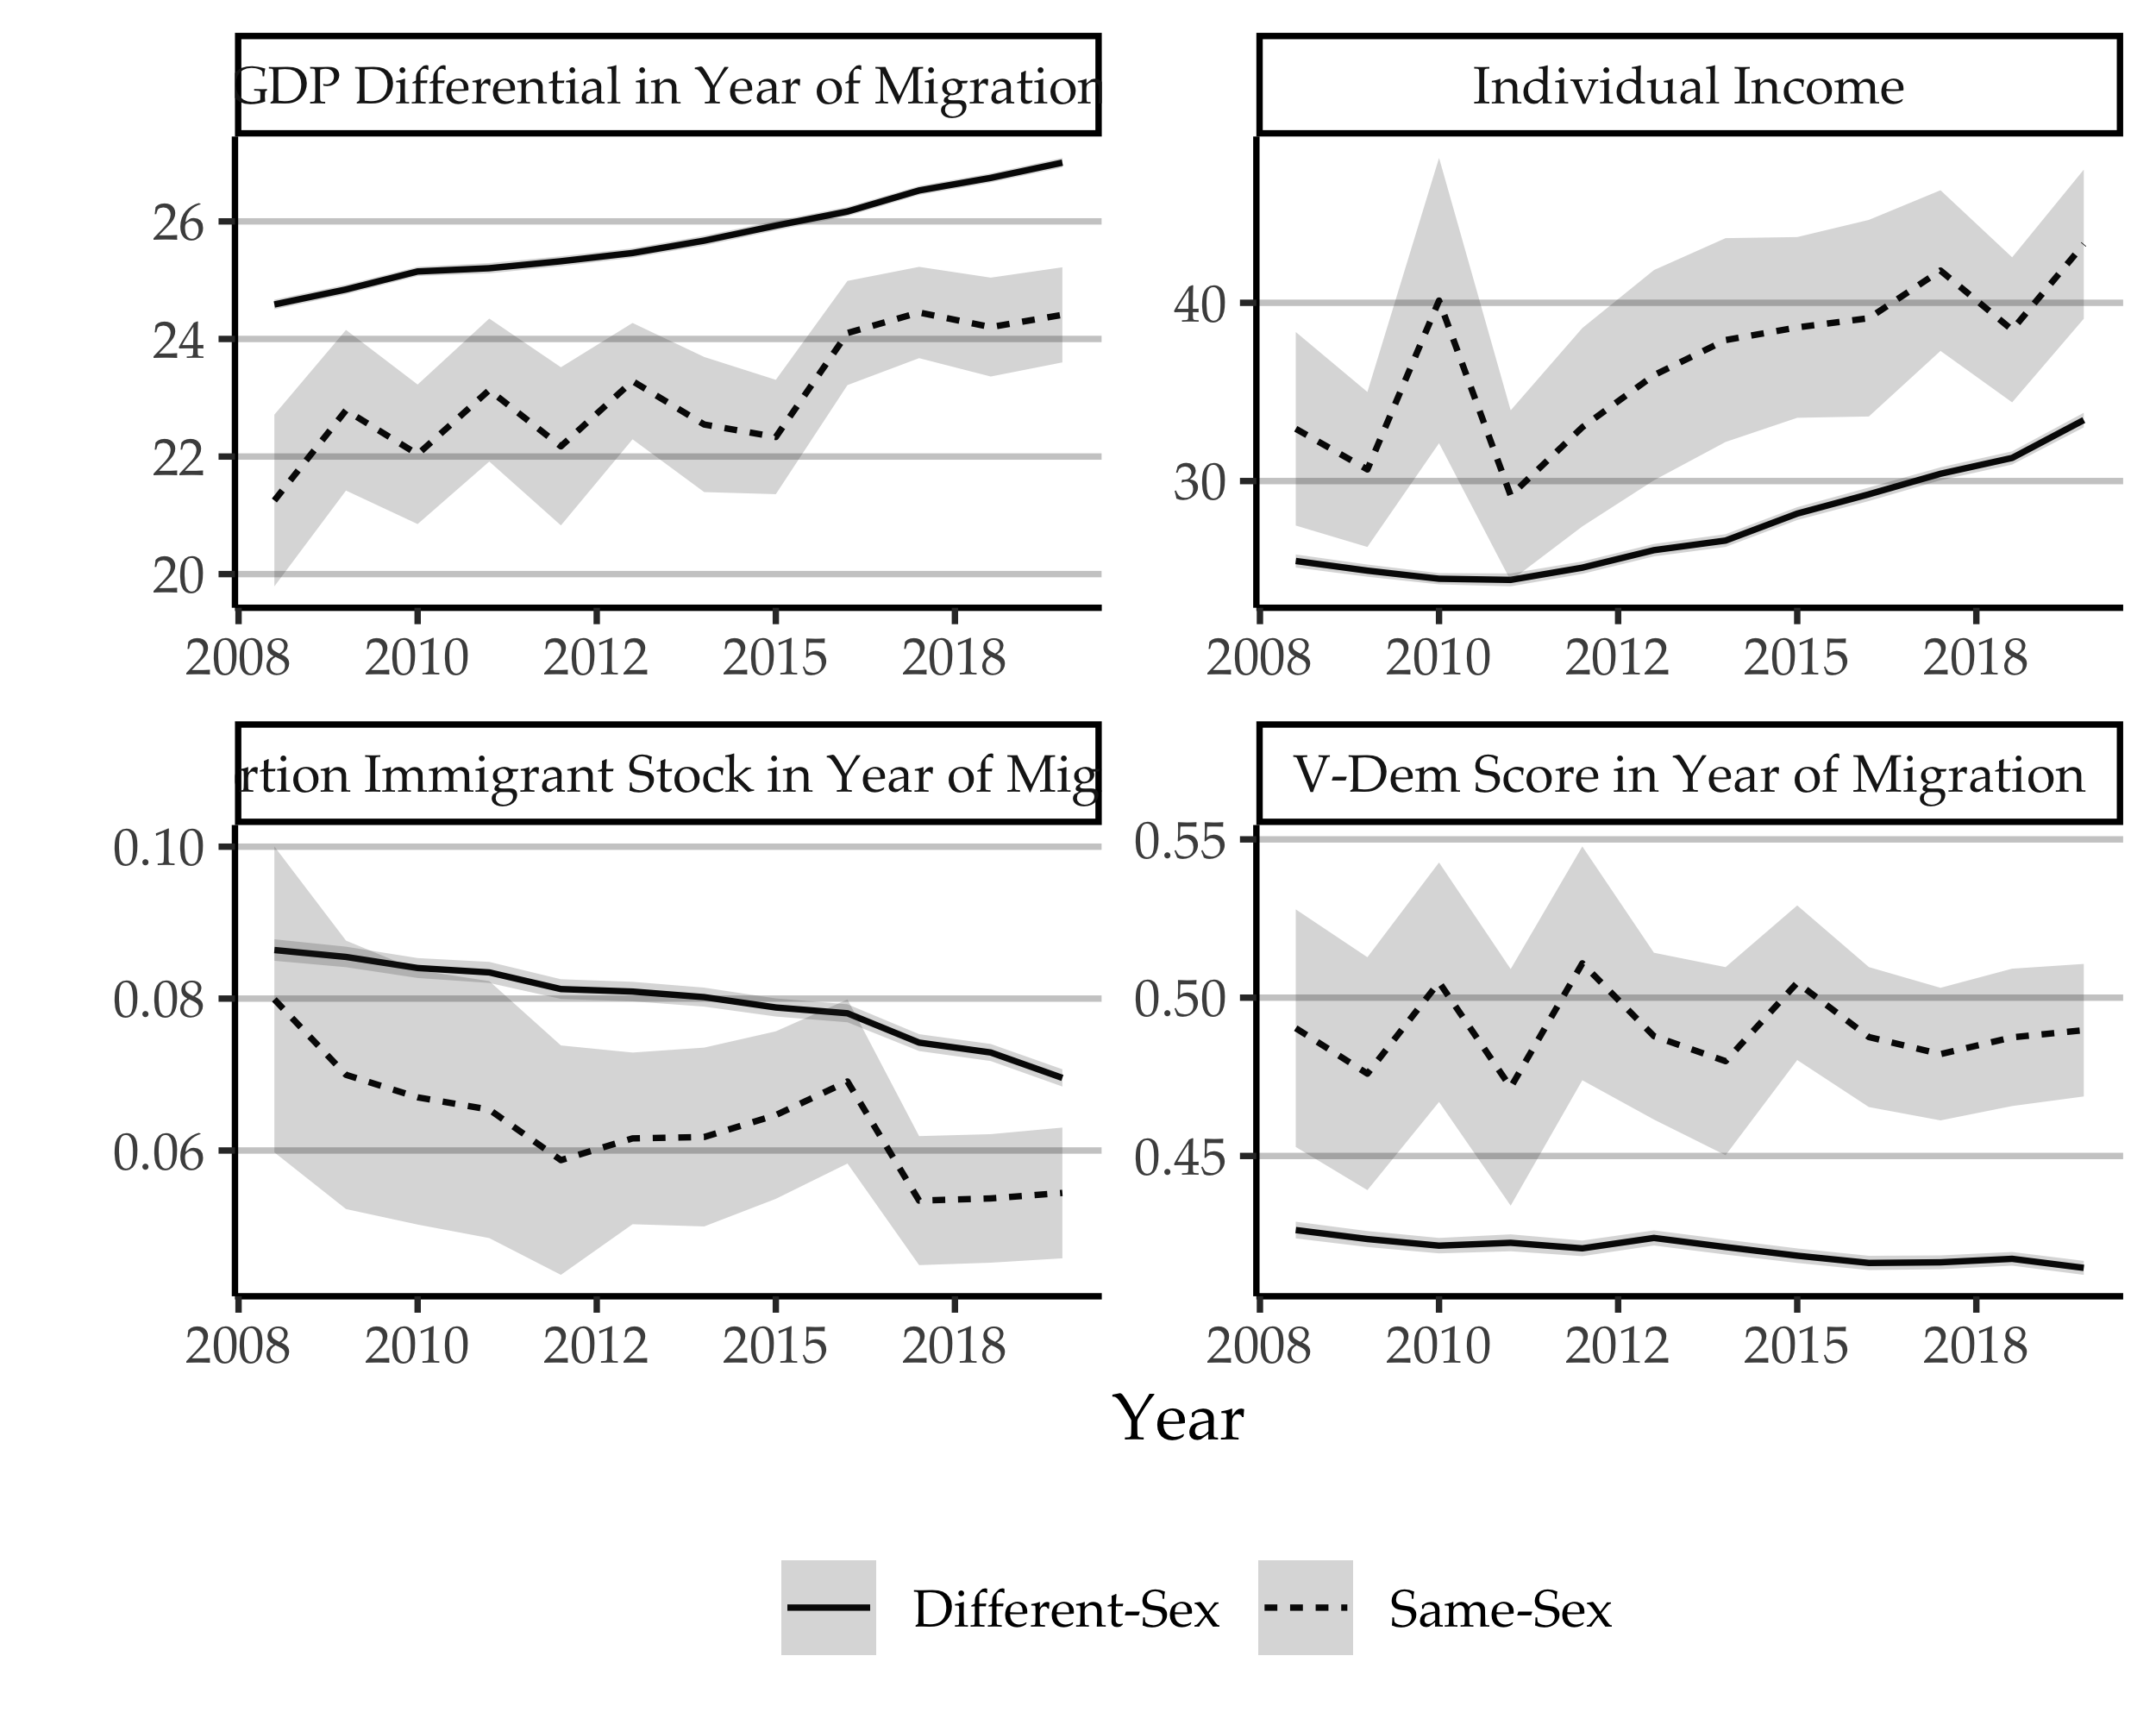
\includegraphics{ssimm_draft_files/figure-latex/desc-1.pdf}
\caption{\label{fig:desc}Descriptive statistics for immigrants in couples 2008-2019, with survey weights and 95\% confidence intervals. All currency in thousands of 1999 dollars.}
\end{figure}

\begin{figure}
\centering
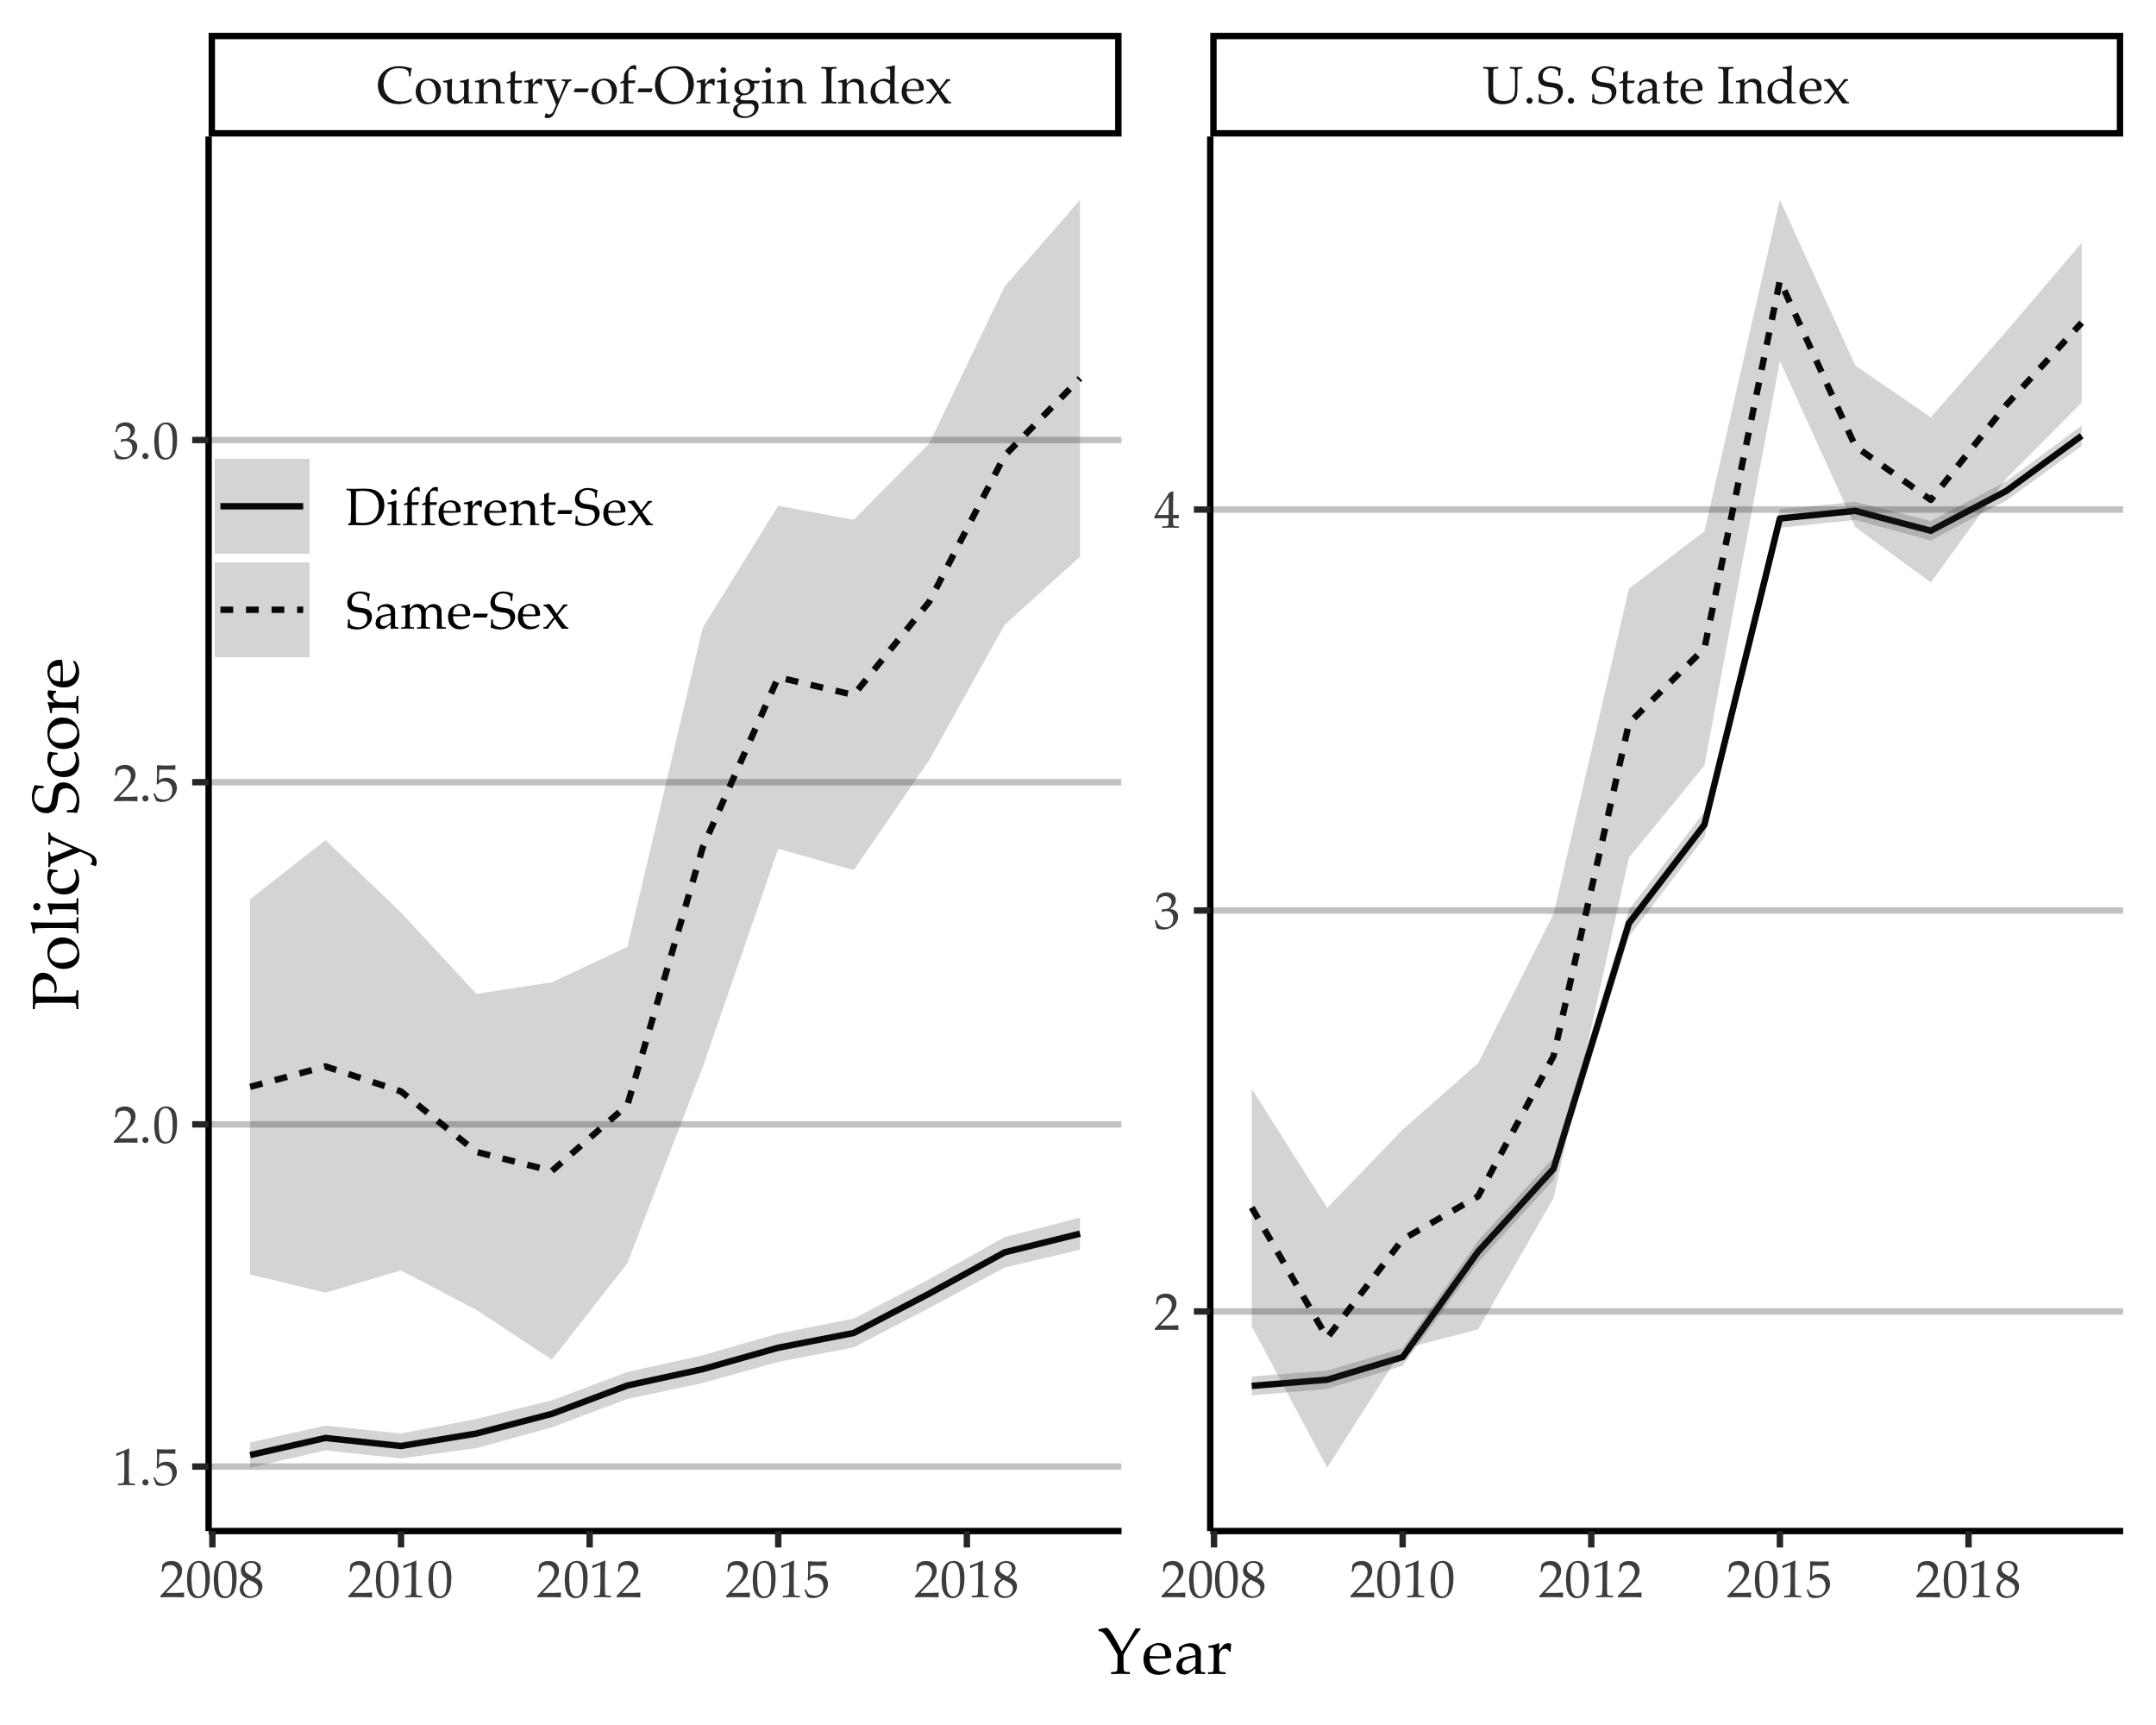
\includegraphics{ssimm_draft_files/figure-latex/policy-desc-1.pdf}
\caption{\label{fig:policy-desc}Mean country-of-origin and U.S. state policy index score for immigrants in same- and different-sex couples, 2008-2019, with 95\% confidence intervals.}
\end{figure}

How do same- and different-sex immigrant couples differ in their individual attributes? Do variables typically used in models for migration differ between the groups? Figure \ref{fig:desc} compares immigrants in same- and different-sex couples on four variables. First, macroeconomic theory predicts that difference in wages and living standards across countries is one of the most important motivations for migration. The first panel in Figure \ref{fig:desc} shows that per-capita GDP is indeed higher in the U.S. than the average country of origin for both groups of immigrants, but the gap is significantly greater for immigrants in different-sex couples. This means that immigrants in same-sex couples are coming from countries with higher standards of living than those in different-sex couples.

Statistics for the unemployment rate differential (see Section B of the Supplementary Material) indicate similar trends: LGB immigrants come from countries with lower unemployment rates. These findings indicate that macroeconomic considerations may be less important to the migration of LGB immigrants. The second panel corroborates this finding on the individual level: Not only do immigrants in same-sex couples come from countries with higher per capita GDP, but they individually tend to earn more than immigrants in different-sex couples. Additional analyses (see Supplementary Material) demonstrate that immigrants in same-sex couples also tend to work in professions with higher occupational prestige scores and have somewhat higher education qualifications, indicating that they may come from more privileged social origins than their heterosexual counterparts.

The bottom-left panel of Figure \ref{fig:desc} looks at a measure of network effects: at the time of immigration, what is the proportion of total immigrants in the U.S. from the country of origin? Compared to different-sex couples, immigrants in same-sex couples immigrated from countries that were less represented in the U.S. population at the time of migration. This indicates that the network effects that attract migrants from the same country of origin may be less relevant to LGB immigrants. Finally, the fourth panel of Figure \ref{fig:desc} compares V-Dem democracy level for country of origin at time of migration. We see that levels of liberal democracy tend to be higher for immigrants in same-sex couples, indicating that political context may play a more important or different role in their migration decisions.

Although we see significant differences between same- and different-sex couples on a number of important migration variables, none shows the sudden jump in recent years reflected in Figure \ref{fig:total-pop}. Turning to LGB policy may better explain this surge. Figure \ref{fig:policy-desc} charts the average country-of-origin and U.S.-state LGB policy score for the immigrants in our sample over time, comparing means for immigrants in same- and different-sex couples. The left panel shows that country-of-origin index at time of migration is generally higher for immigrants in same-sex couples, and since 2013 it has rapidly increased. Immigrants in same-sex couples tend to come from more progressive countries, and this trend tracks closely with the overall population of this group. The right panel indicates less of a difference in U.S. state policies, although states where immigrants in same-sex couples live tend to score somewhat higher.

\begin{figure}
\centering
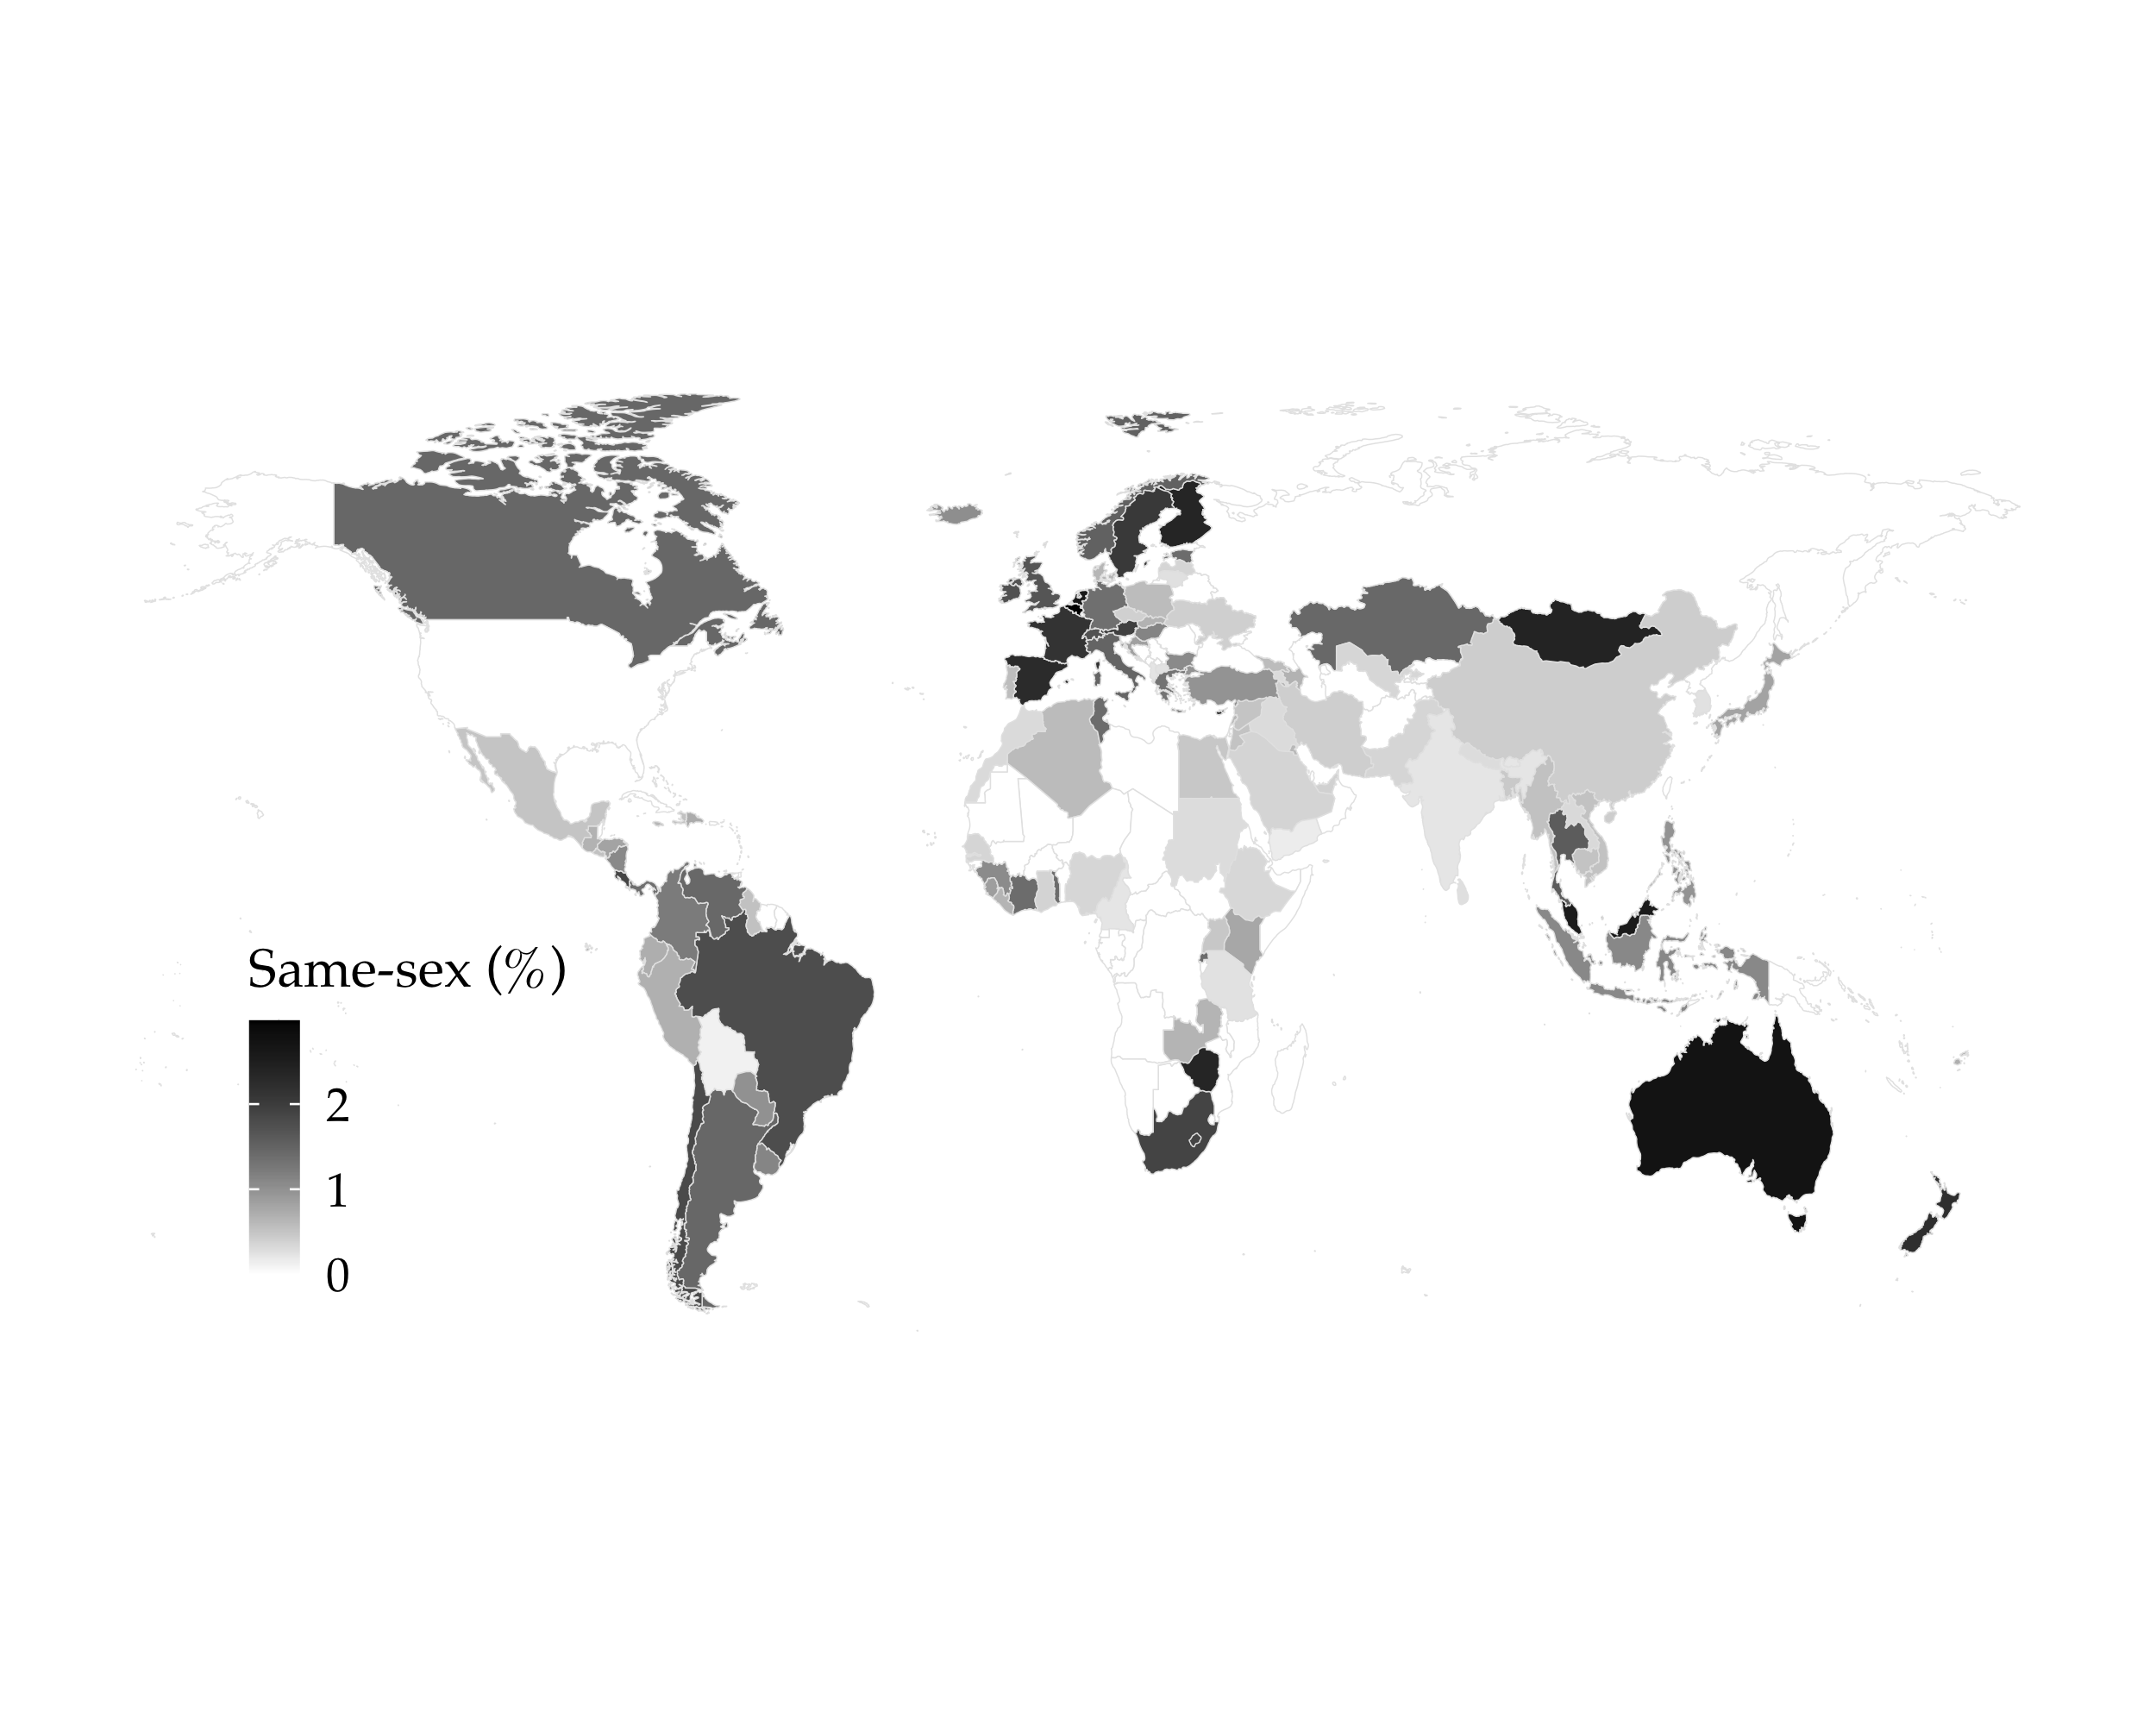
\includegraphics{ssimm_draft_files/figure-latex/country-map-1.pdf}
\caption{\label{fig:country-map}Percentage of immigrants to the U.S. in same-sex couples by country of origin, averaging over years of immigration from 1991 to 2019.}
\end{figure}

\begin{figure}
\centering
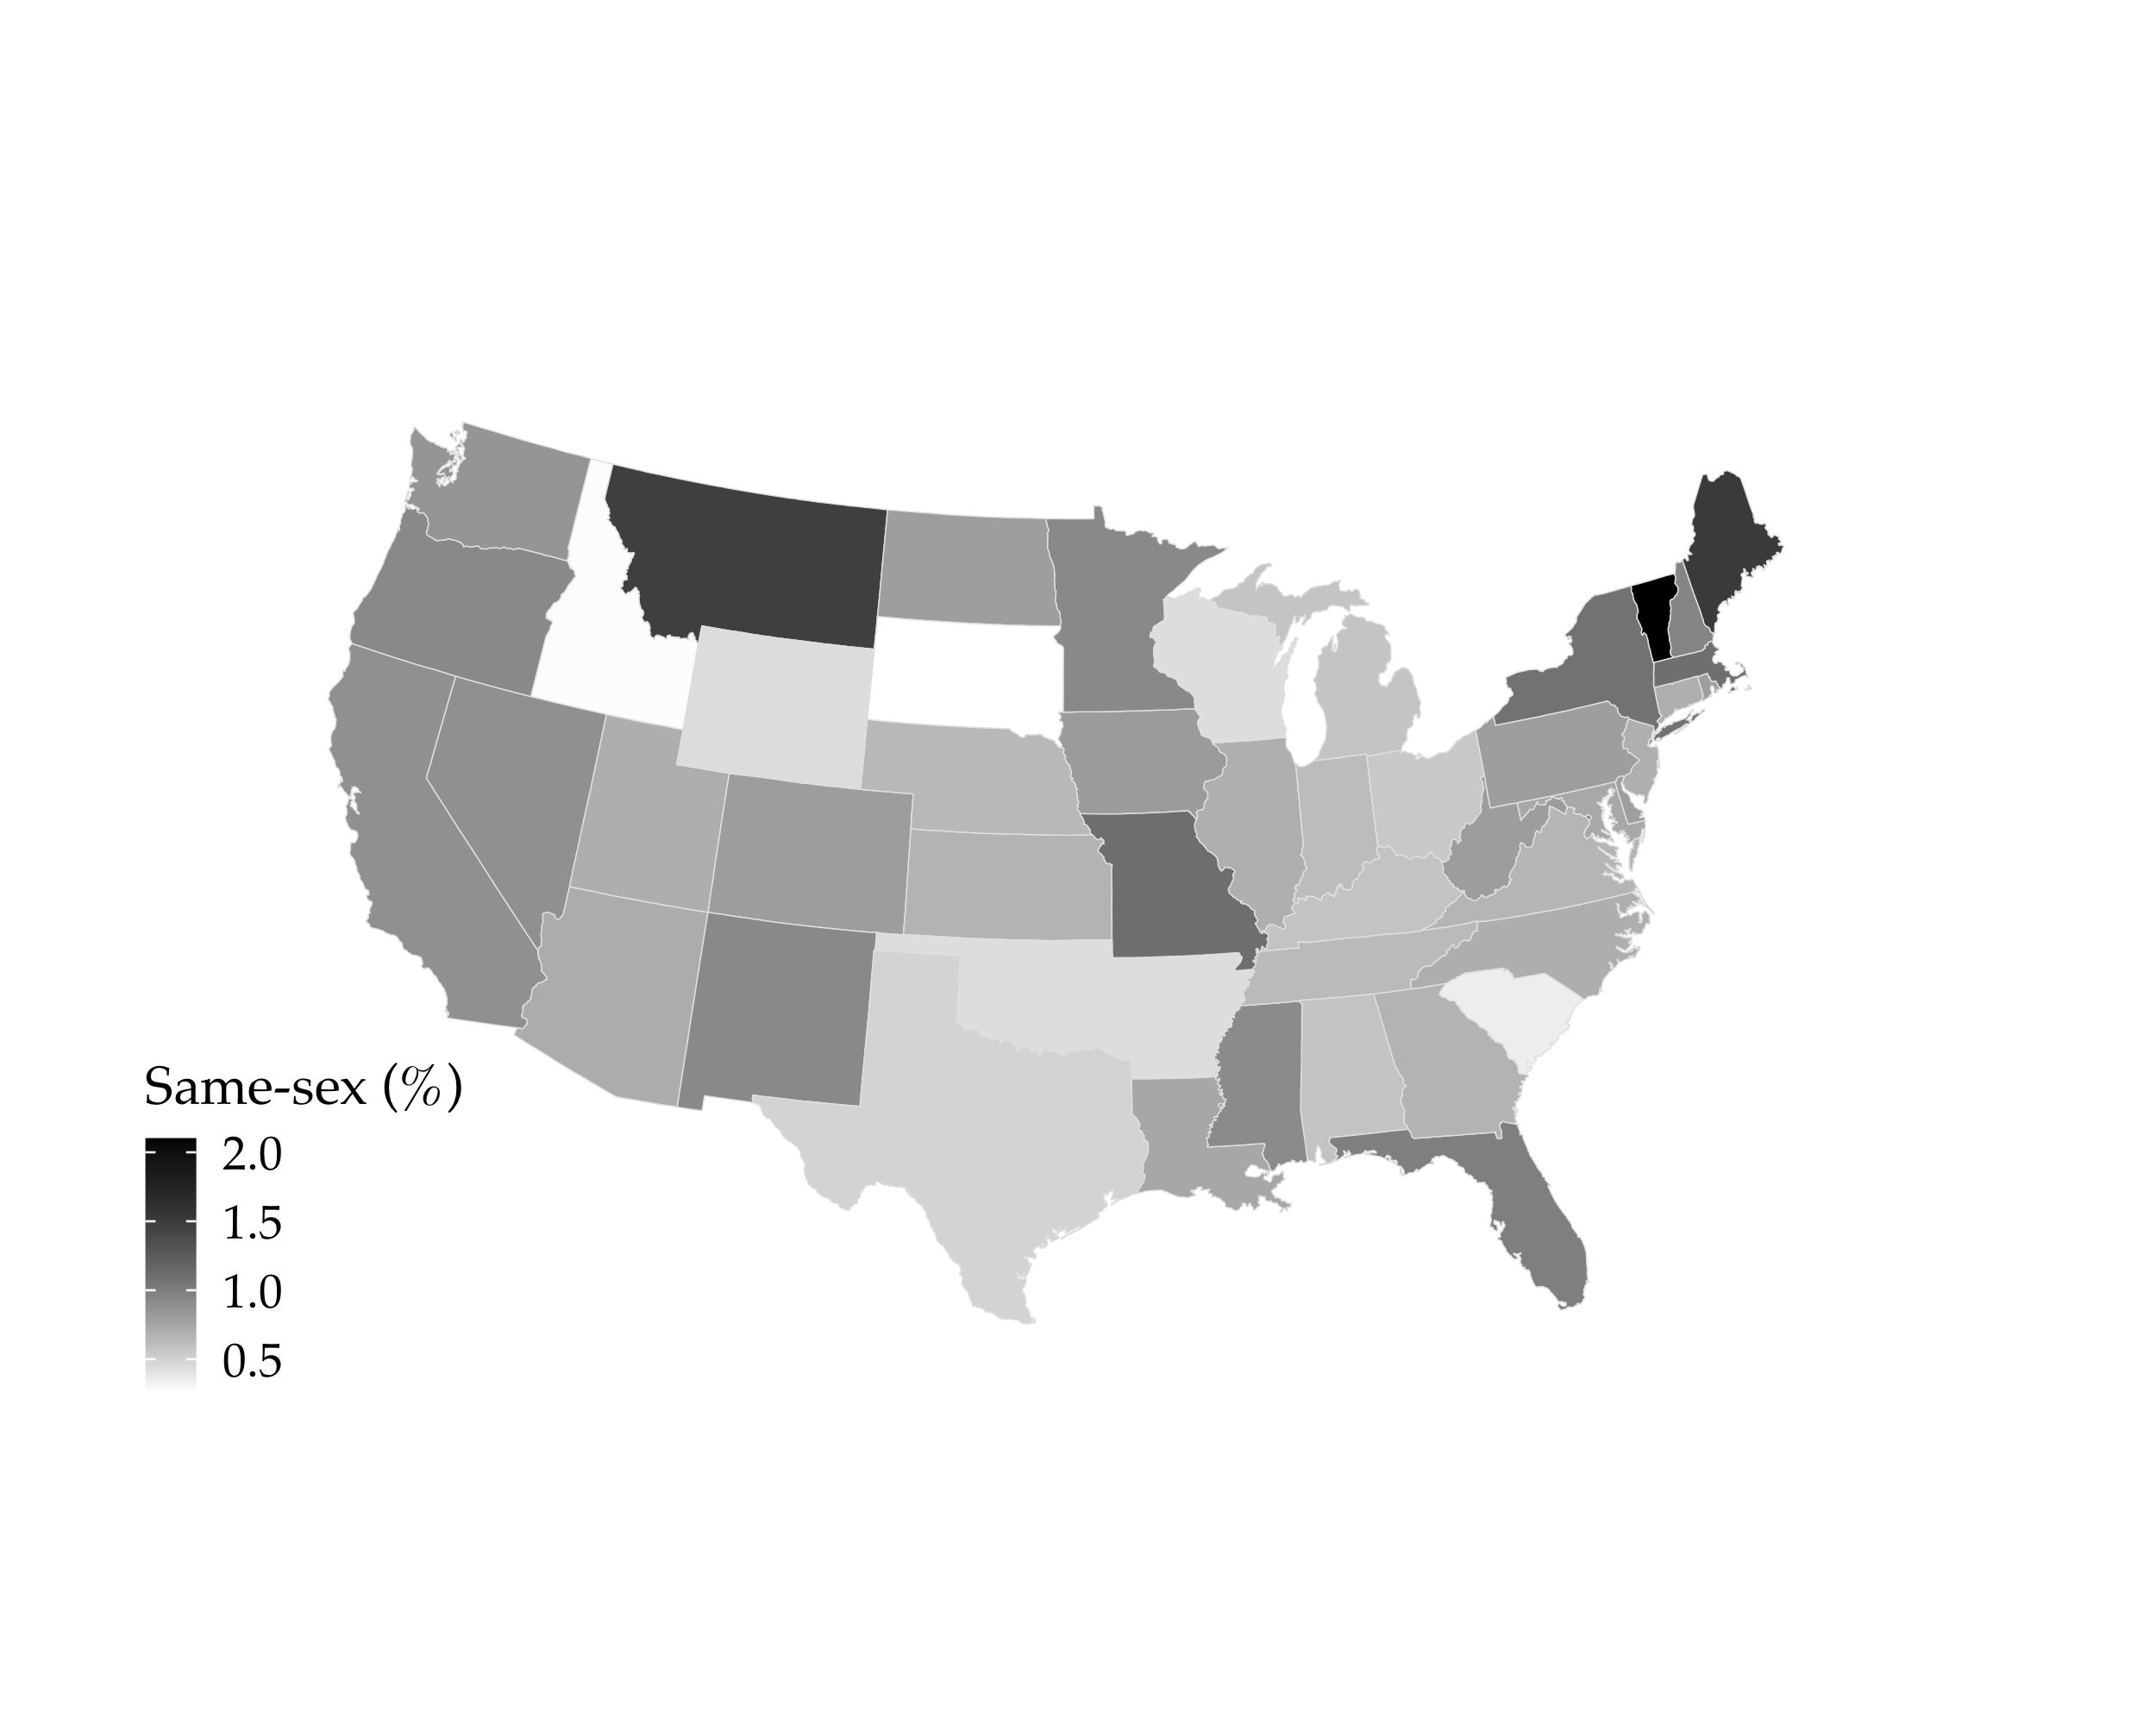
\includegraphics{ssimm_draft_files/figure-latex/state-map-1.pdf}
\caption{\label{fig:state-map}Percentage of immigrants in same-sex couples in U.S. states, averaging over ACS survey years 2008 to 2019.}
\end{figure}

Figure \ref{fig:country-map} shows the percentage of immigrants to the U.S. in same-sex couples from each country of origin, averaging over the 29 possible years of immigration, and Table \ref{tab:country-tab} presents the top ten of these along with average LGB policy score over these years. The top sending countries include interesting diversity. Although countries with more progressive policies top the list, Malaysia, Zimbabwe, and Singapore make the list with their relatively repressive contexts. Having countries within the top 10 span multiple regions and cultures provides preliminary evidence that LGB policy in not substantially affecting willingness to respond truthfully on the ACS about being in a same-sex couple. Nor does it appear as though responses to the ACS are simply a function of country-of-origin LGB policies, as policy scores vary significantly across the top 10. Figure \ref{fig:state-map} presents the percentage of immigrants in same-sex couples in U.S. states, averaging over the survey years and possible countries of origin, and Table \ref{tab:state-tab} ranks the top ten. Although states with progressive policies occupy the top spots, Montana, Missouri, and Florida still make the list with less affirming policy environments.

\begin{table}

\caption{\label{tab:country-tab}Sending countries ranked by proportion immigrant couples with same-sex partners}
\centering
\begin{tabular}[t]{lllr}
\toprule
Rank & Country of origin & Proportion same-sex & Mean policy score\\
\midrule
1 & Belgium & 2.98 \% & 5.38\\
2 & Australia & 2.73 \% & 4.56\\
3 & Netherlands & 2.61 \% & 7.20\\
4 & Malaysia & 2.56 \% & -1.01\\
5 & Mongolia & 2.41 \% & 2.15\\
6 & Zimbabwe & 2.38 \% & -1.07\\
7 & Finland & 2.37 \% & 4.42\\
8 & Singapore & 2.34 \% & -0.02\\
9 & Cyprus & 2.30 \% & 0.66\\
10 & Spain & 2.27 \% & 6.33\\
\bottomrule
\multicolumn{4}{l}{\rule{0pt}{1em}\textit{Source:} American Community Survey 2008-2019. Authors' calculations.}\\
\end{tabular}
\end{table}

\begin{table}

\caption{\label{tab:state-tab}States ranked by proportion immigrant couples with same-sex partners}
\centering
\begin{tabular}[t]{lllr}
\toprule
Rank & State & Proportion same-sex & Mean policy score\\
\midrule
1 & Vermont & 2.10 \% & 5.25\\
2 & Maine & 1.51 \% & 4.85\\
3 & Montana & 1.47 \% & 0.93\\
4 & Missouri & 1.11 \% & 1.96\\
5 & Massachusetts & 1.10 \% & 4.80\\
6 & New York & 1.08 \% & 4.89\\
7 & Florida & 0.99 \% & 1.00\\
8 & New Hampshire & 0.95 \% & 4.40\\
9 & Minnesota & 0.92 \% & 4.66\\
10 & New Mexico & 0.92 \% & 4.80\\
\bottomrule
\multicolumn{4}{l}{\rule{0pt}{1em}\textit{Source:} American Community Survey 2008-2019. Authors' calculations.}\\
\end{tabular}
\end{table}

\hypertarget{model-results}{%
\subsection{Model Results}\label{model-results}}

\hypertarget{country-of-origin-effects}{%
\subsubsection{Country-of-Origin Effects}\label{country-of-origin-effects}}

Our first set of models predicts the percent of immigrants in same-sex couples by country of origin and year of immigration (Table \ref{tab:country-props}). Model 1 regresses this proportion on only our variable of interest, LGB policy score in country of origin. We see that countries with more progressive LGB policies tend to send more immigrants to the U.S. who end up in same-sex couples. The average country-level proportion of immigrants in same-sex couples is only 0.46 percent, so an increase of 0.088 percent per point increase in LGB policy score represents a substantial effect. Models 2 and 3 in Table \ref{tab:country-props} assess the robustness of this finding. Model 2 includes typical migration controls, including economic differentials, distance, immigrant networks, and democracy. Model 3 adds country-of-origin fixed effects. Although in this model coefficient for origin score is reduced compared to Model 1, it remains statistically significant.

\begin{table}[!htbp] \centering 
  \caption{OLS regressions of percent of immigrants in same-sex couples by year of immigration and country of origin.} 
  \label{tab:country-props} 
\begin{tabular}{@{\extracolsep{5pt}}lccccc} 
\\[-1.8ex]\hline 
\hline \\[-1.8ex] 
 & \multicolumn{5}{c}{\textit{Dependent variable:}} \\ 
\cline{2-6} 
\\[-1.8ex] & \multicolumn{5}{c}{Percent in same-sex couples by country-year} \\ 
\\[-1.8ex] & (1) & (2) & (3) & (4) & (5)\\ 
\hline \\[-1.8ex] 
 Country LGB policy score & 0.088$^{***}$ & 0.052$^{***}$ & 0.051$^{*}$ & 0.023 & $-$0.019 \\ 
  & (0.012) & (0.015) & (0.023) & (0.025) & (0.029) \\ 
  & & & & & \\ 
 Post-2013 &  &  &  & 0.280$^{**}$ & 0.130 \\ 
  &  &  &  & (0.088) & (0.100) \\ 
  & & & & & \\ 
 Country score × Post-2013 &  &  &  &  & 0.074$^{**}$ \\ 
  &  &  &  &  & (0.026) \\ 
  & & & & & \\ 
\hline \\[-1.8ex] 
Country controls? & no & yes & yes & yes & yes \\ 
Country FEs? & no & no & yes & yes & yes \\ 
Observations & 3,281 & 3,281 & 3,281 & 3,281 & 3,281 \\ 
\hline 
\hline \\[-1.8ex] 
\multicolumn{6}{l}{\parbox[t]{.8\textwidth}{\textit{Note}: †\textit{p}<0.1; *\textit{p}<0.05; **\textit{p}<0.01; ***\textit{p}<0.001. Country-clustered standard errors shown in parentheses. Country controls include population-weighted distance, contiguous border, common official language, common ethnic language, colonial relationship, per-capita GDP differential, unemployment differential, proportion same-country stock, and democracy.}} \\ 
\multicolumn{6}{l}{\textit{Source}: American Community Survey 2008-2019} \\ 
\end{tabular} 
\end{table}

In light of the 2013 Supreme Court decision striking down DOMA, Models 4 and 5 assess how these processes have changed since 2013. Model 4 is the same as Model 3, but with a dichotomous ``Post-2013'' variable added. The influence of sending-country policy loses its significance in this model: 2013 was a significant turning point for LGB immigrants to the U.S., with the average representation from a given country growing by a quarter of a percent. Model 5 adds an interaction between sending-country LGB policy score and the post-2013 dichotomous variable. This variable is significant and positive, while the other variables of interest lose significance. Sending-country policy and the post-2013 era both matter, but solely in tandem: Only LGB immigrants from progressive countries see a boost in representation after the DOMA decision.

\hypertarget{state-effects}{%
\subsubsection{State Effects}\label{state-effects}}

\begin{table}[!htbp] \centering 
  \caption{Percent same-sex in by country of origin, U.S. state, and survey year.} 
  \label{tab:state-props} 
\begin{tabular}{@{\extracolsep{5pt}}lccccccc} 
\\[-1.8ex]\hline 
\hline \\[-1.8ex] 
 & \multicolumn{7}{c}{\textit{Dependent variable:}} \\ 
\cline{2-8} 
\\[-1.8ex] & \multicolumn{7}{c}{Percent in same-sex couples by state-country-year} \\ 
\\[-1.8ex] & (1) & (2) & (3) & (4) & (5) & (6) & (7)\\ 
\hline \\[-1.8ex] 
 State LGB policy score & 0.055$^{***}$ & 0.052$^{***}$ & 0.097$^{**}$ & 0.078$^{*}$ & 0.066$^{†}$ & 0.064$^{†}$ & 0.067$^{†}$ \\ 
  & (0.010) & (0.010) & (0.034) & (0.034) & (0.037) & (0.038) & (0.037) \\ 
  & & & & & & & \\ 
 Country LGB policy score &  & 0.086$^{***}$ & 0.130$^{**}$ & 0.077 & 0.120$^{**}$ & 0.120$^{**}$ & 0.015 \\ 
  &  & (0.010) & (0.044) & (0.047) & (0.044) & (0.044) & (0.053) \\ 
  & & & & & & & \\ 
 State score × country-score &  &  &  & 0.013$^{**}$ &  &  &  \\ 
  &  &  &  & (0.004) &  &  &  \\ 
  & & & & & & & \\ 
 Post-2013 &  &  &  &  & 0.190$^{*}$ & 0.180$^{†}$ & 0.077 \\ 
  &  &  &  &  & (0.094) & (0.100) & (0.100) \\ 
  & & & & & & & \\ 
 State score × post-2013 &  &  &  &  &  & 0.004 &  \\ 
  &  &  &  &  &  & (0.022) &  \\ 
  & & & & & & & \\ 
 Country score × post-2013 &  &  &  &  &  &  & 0.079$^{***}$ \\ 
  &  &  &  &  &  &  & (0.023) \\ 
  & & & & & & & \\ 
\hline \\[-1.8ex] 
State controls and FEs? & no & no & yes & yes & yes & yes & yes \\ 
Country controls and FEs? & no & no & yes & yes & yes & yes & yes \\ 
Observations & 35,868 & 35,868 & 35,868 & 35,868 & 35,868 & 35,868 & 35,868 \\ 
\hline 
\hline \\[-1.8ex] 
\multicolumn{8}{l}{\parbox[t]{\textwidth}{\textit{Note}: †\textit{p}<0.1; *\textit{p}<0.05; **\textit{p}<0.01; ***\textit{p}<0.001. Country and state two-way clustered standard errors are shown in parentheses. State controls include unemployment rate and per-capita income. Country controls include population-weighted distance, contiguous border, common official language, common ethnic language, colonial relationship, per-capita GDP differential, unemployment differential, proportion same-country stock, and democracy.}} \\ 
\multicolumn{8}{l}{\textit{Source}: American Community Survey 2008-2019} \\ 
\end{tabular} 
\end{table}

We next turn to the effects of U.S. state LGB policy. Table \ref{tab:state-props} presents models of the U.S. state-level proportion of immigrants in same-sex couples, from a given country of origin in a given survey year. Model 1 contains only one predictor: U.S. state policy score in the survey year. We see that, on average, states with more friendly LGB policies have somewhat higher proportions of immigrants in same-sex couples. Model 2 adds a predictor for country-of-origin policy score at the mean year of immigration. Although the coefficient for country of origin score is more precisely estimated, the two variables have effects of roughly equal size. A one-standard deviation (2-point) increase origin score is associated with a 0.17 percentage-point increase of immigrants in same-sex couples, whereas the corresponding state policy standard deviation increase of 2.4 points is 0.13 percentage points.

According to the descriptive analysis above, immigrants in same-sex couples tend to have higher incomes and hold more prestigious occupations than immigrants in different-sex couples, and they tend to come from wealthier countries. This implies that immigrants in same-sex couples may be attracted to progressive states for their economic rather than political benefits, so Model 3 adds state and origin-country controls and fixed effects. Surprisingly, the coefficients for state score and country score \emph{grow} in strength. More progressive sending countries are represented by greater proportions of same-sex couples, and they tend to settle in more progressive U.S. states.

Model 4 adds an interaction between state and country LGB scores. It is positive and significant, and the coefficient for state score retains its value while that for country score becomes insignificant. Progressive states attract higher proportions of same-sex immigrant couples, and this effect is stronger for immigrants from more progressive countries.

Finally, Model 5 includes a dichotomous variable for the post-2013 DOMA decision era, and Models 6 and 7 interact this with state and sending-country scores, respectively. The significant post-2013 variable in Model 5 implies that proportions LGB have increased across the country in the past few years. Coefficients for state policy, including in its interaction with the post-2013 dichotomous variable, become less important in these models, whereas origin-country score retains its effect. After 2013, the proportion of immigrants in same-sex couples increased across states for those from more progressive countries. With increasingly progressive federal policy, state policy appears to matter less in the post-DOMA era.

\hypertarget{individual-analysis}{%
\subsubsection{Individual Analysis}\label{individual-analysis}}

Our final set of models focuses on the individual. Conditional on migrating to the U.S., do immigrants in same-sex couples choose to live in more progressive states than their heterosexual counterparts? Table \ref{tab:ord} presents ordered logit models predicting whether an individual partnered immigrant lives in a U.S. state with repressive, neutral, or progressive LGB policies, pooling data across survey years. Model 1 includes only one regressor: an indicator for whether the immigrant is in a same-sex couple. The positive coefficient indicates that immigrants in same-sex couples indeed tend to live in states with more LGB-friendly policies. The predicted probability for an immigrant in a different-sex couple to live in a state with progressive LGB policies is 0.59, whereas the corresponding probability for those in same-sex couples rises to 0.67. The repressive end of the policy spectrum shows reversed trends: The predicted probabilities for living in a progressive state are 0.21 and 0.16 for different- and same-sex couples, respectively.

How does country-of-origin context mediate these results? Model 2 adds sending-country LGB policy score at the time of immigration to the regression, interacting it with the same-sex indicator. The coefficient for the same-sex indicator remains positive and significant, but we see opposite effects of the origin-score coefficient for immigrants in different- and same-sex couples. For different-sex couples, hailing from a more progressive country is associated with living in a more repressive U.S. state. For same-sex couples, the result is in the opposite direction: Those from progressive countries tend to live in more progressive U.S. states.

Model 3 controls for possible individual confounders, interacting them with the same-sex indicator. If immigrants in same-sex couples also tend to be more educated, earn higher wages, have different family structures, or be younger, they may be choosing more progressive states due to other policies or economic conditions. Yet our variables of interest remain strong and in the same directions in this model. Since correlated aspects of sending country and state or residence may be confounding our results, our final individual model adds state and country controls. The coefficient for sending country becomes very small, and although they shrink in size, the same-sex coefficient and interaction remain significant. These results are in line with results in Table \ref{tab:state-props}: Same-sex couples are more likely to live in progressive states, and although origin-country score has no relationship with different-sex couples' state policy environment, same-sex couples hailing from more progressive countries are even more likely to live in progressive states.

\begin{table}[!htbp] \centering 
  \caption{Individual ordered logit analysis of three-category state policy score.} 
  \label{tab:ord} 
\begin{tabular}{@{\extracolsep{5pt}}lcccc} 
\\[-1.8ex]\hline 
\hline \\[-1.8ex] 
 & \multicolumn{4}{c}{\textit{Dependent variable:}} \\ 
\cline{2-5} 
\\[-1.8ex] & \multicolumn{4}{c}{Binned state LGB policy score} \\ 
\\[-1.8ex] & (1) & (2) & (3) & (4)\\ 
\hline \\[-1.8ex] 
 Same-sex & 0.350$^{***}$ & 0.250$^{***}$ & 23.000$^{***}$ & 15.000$^{***}$ \\ 
  & (0.009) & (0.012) & (0.00000) & (0.00000) \\ 
  & & & & \\ 
 Country LGB policy score &  & $-$0.041$^{***}$ & $-$0.048$^{***}$ & $-$0.003$^{***}$ \\ 
  &  & (0.0003) & (0.0003) & (0.001) \\ 
  & & & & \\ 
 Same-sex × country score &  & 0.054$^{***}$ & 0.050$^{***}$ & 0.008$^{***}$ \\ 
  &  & (0.003) & (0.00004) & (0.00002) \\ 
  & & & & \\ 
\hline \\[-1.8ex] 
Individual controls? & no & no & yes & yes \\ 
State and country controls? & no & no & no & yes \\ 
Observations & 905,880 & 905,880 & 905,880 & 905,880 \\ 
\hline 
\hline \\[-1.8ex] 
\multicolumn{5}{l}{\parbox[t]{.8\textwidth}{\textit{Note}: †\textit{p}<0.1; *\textit{p}<0.05; **\textit{p}<0.01; ***\textit{p}<0.001. Country and state two-way clustered standard errors are shown in parentheses. Individual controls include sex, age, education, number of children, IHS-transformed income, indicator for no income, and year of immigration, which are all interacted with the indicator for same-sex couple. State controls include unemployment rate and per-capita income. Country controls include population-weighted distance, contiguous border, common official language, common ethnic language, colonial relationship, per-capita GDP differential, unemployment differential, proportion same-country stock, and democracy.}} \\ 
\multicolumn{5}{l}{\textit{Source}: American Community Survey 2008-2019} \\ 
\end{tabular} 
\end{table}

We put these results into perspective using simulated probabilities over the entire sample, varying each individual's same-sex indicator and origin-country LGB score. At the high end of the origin-score policy range, typical immigrants in same-sex couples are 3.4 percentage points more likely to live in progressive states and 2.8 percentage points less likely to live in repressive states than similar immigrants in different-sex couples. These results demonstrate that sexuality, and the governance of it, are closely related to migration patterns for those in same-sex relationships.

\hypertarget{robustness-checks}{%
\subsection{Robustness Checks}\label{robustness-checks}}

\begin{figure}
\centering
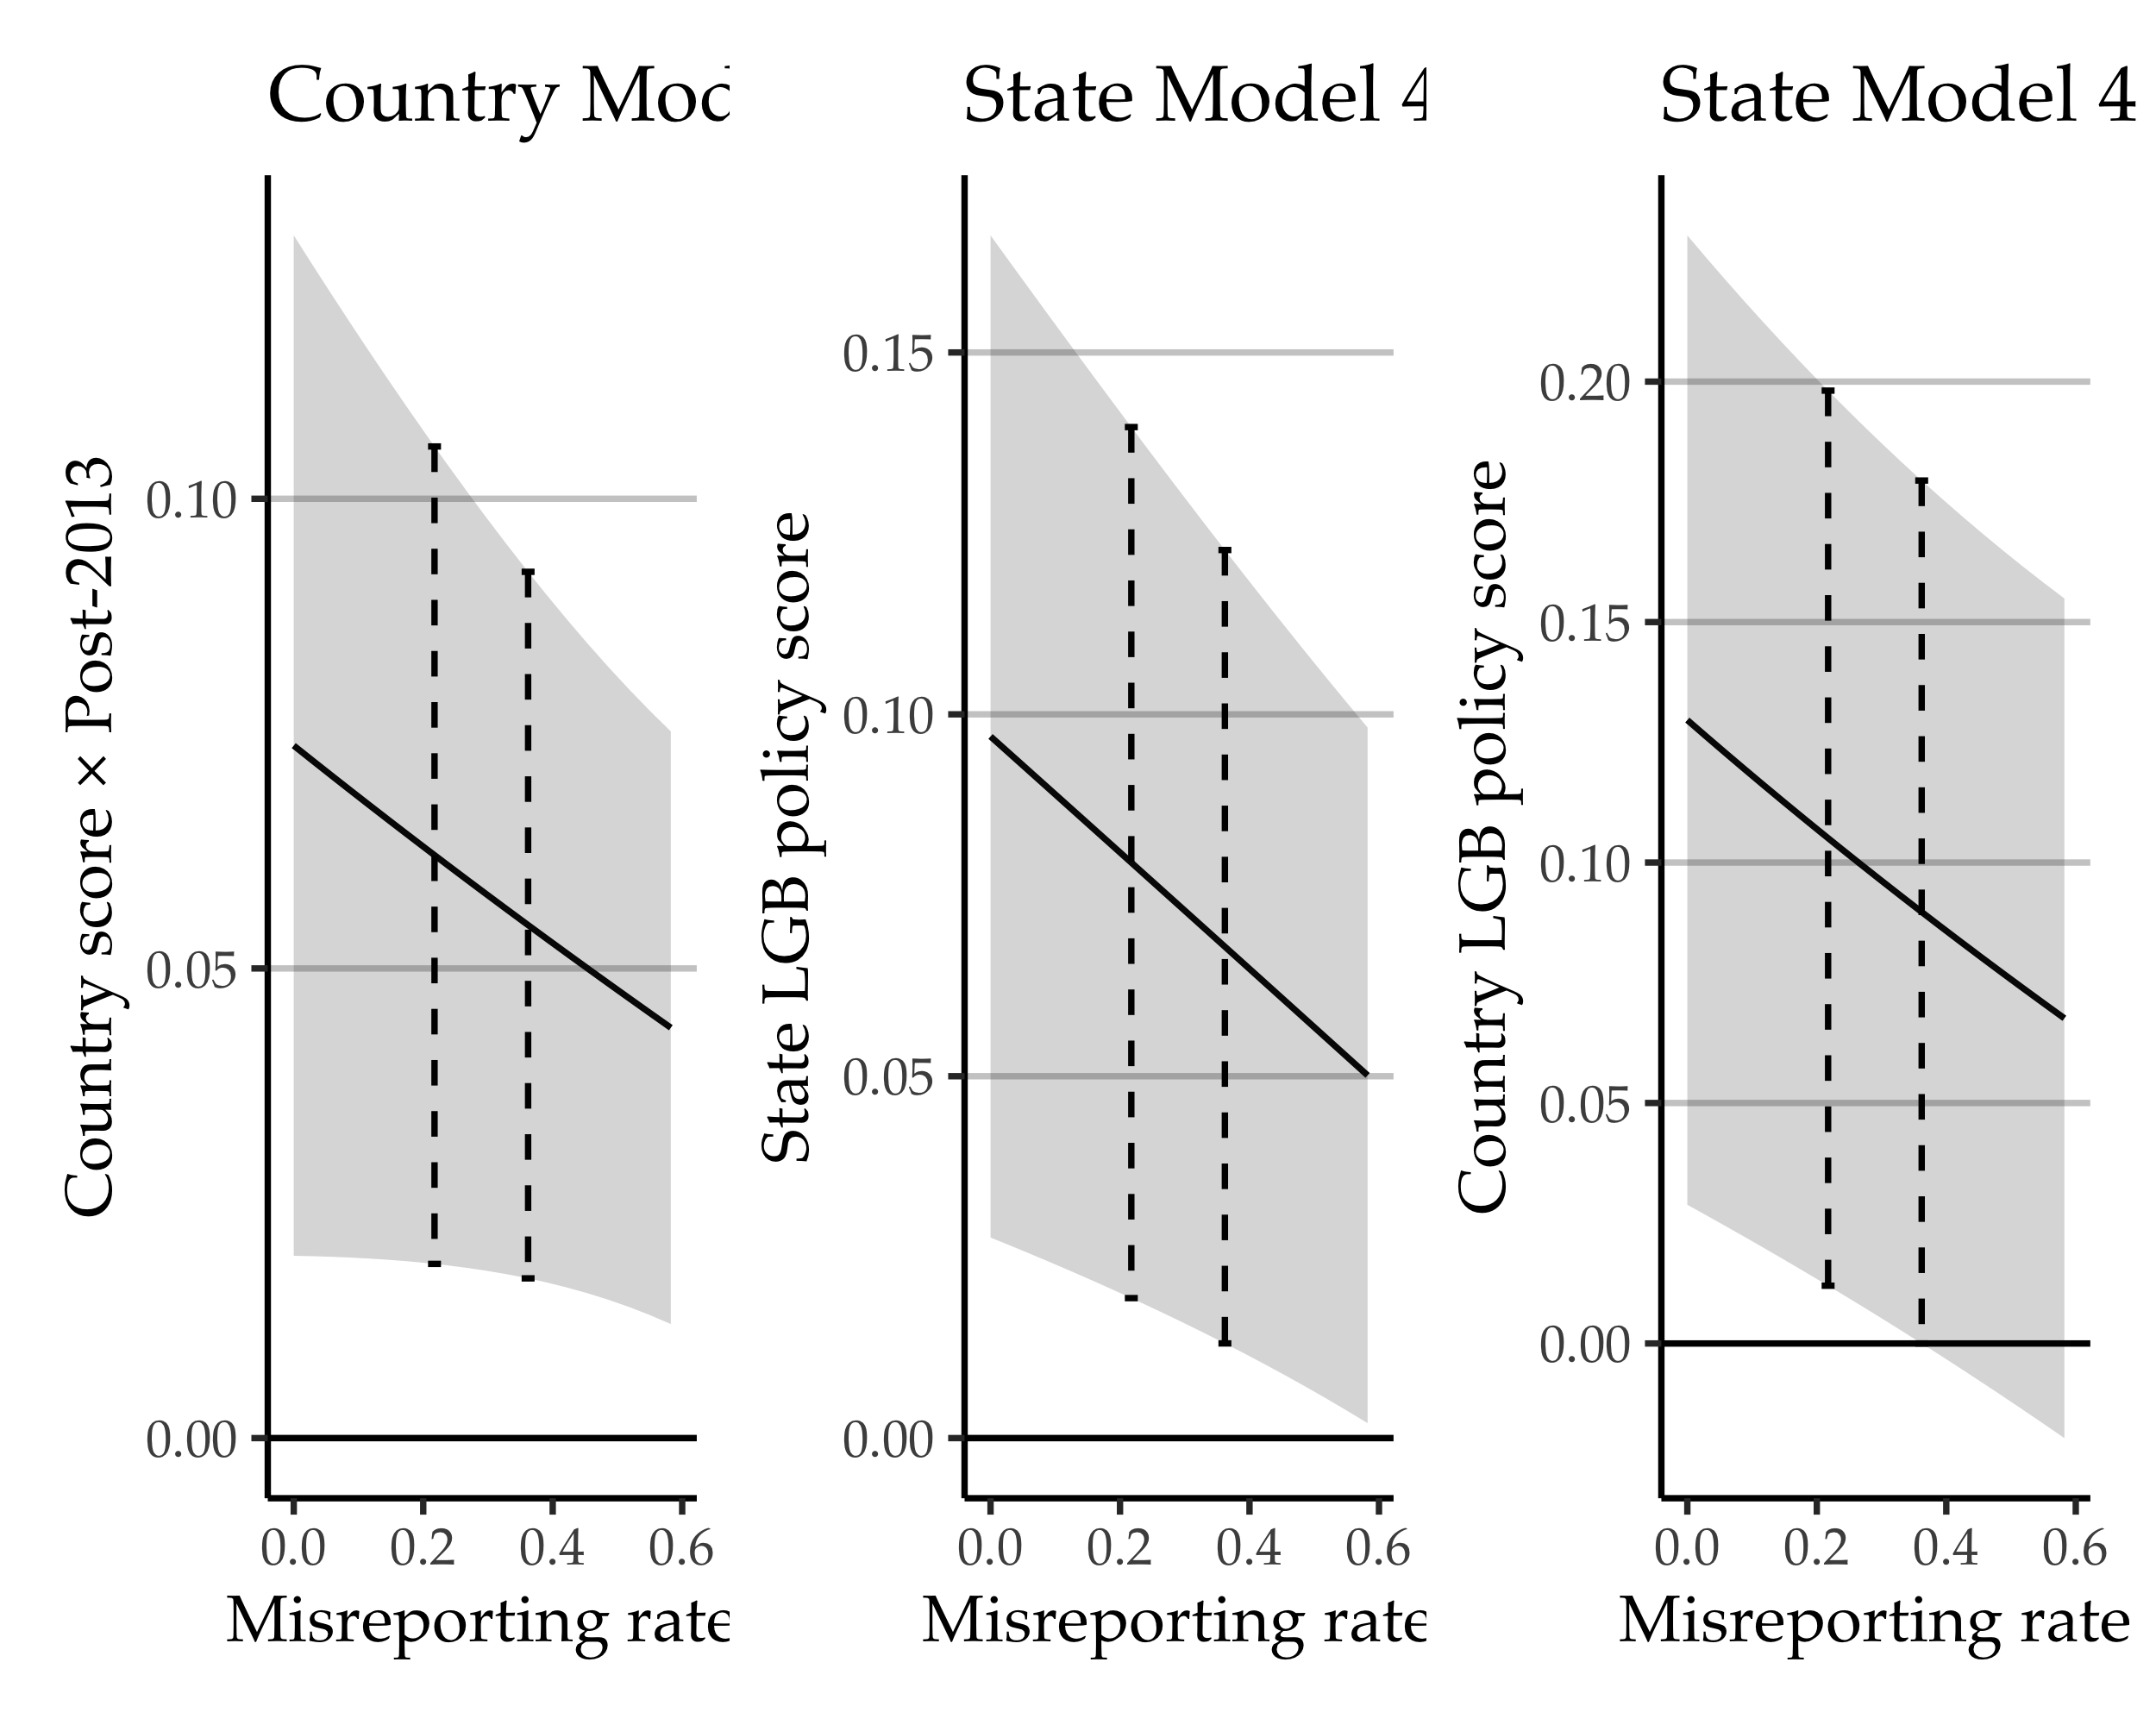
\includegraphics{ssimm_draft_files/figure-latex/sens-1.pdf}
\caption{\label{fig:sens}Coefficients for sending-country and U.S. state LGB policy context for fixed effects models in Tables 3 and 4, adjusted for hypothetical misreporting rates of married and unmarried same-sex couples in pre-2019 data. Ribbon shows 95 percent confidence intervals and dashed bars show estimated misreporting from the 2010 and 2016 U.S. Census Bureau tests on the ACS.}
\end{figure}

Our results hold up to a variety of robustness checks presented in Section C of the Supplementary Material; we outline the major results here. First, as mentioned above, sex misreporting may bias the results by including a non-trivial number of different-sex couples in the counts of same-sex couples. Published papers using the ACS to study same-sex couples overwhelmingly deal with potential misreporting using the method suggested by \protect\hyperlink{ref-gates_2009}{Gates \& Steinberger} (\protect\hyperlink{ref-gates_2009}{2009}) that we employ: dropping respondents whose sex or relation to household head were allocated by the Census Bureau. We conduct a more stringent test of the sensitivity of our results to misreporting, using the empirical mismatch rates by survey response mode from two studies conducted by the Census Bureau in 2010 and 2016 (\protect\hyperlink{ref-kreider_2017}{Kreider et al., 2017}; \protect\hyperlink{ref-kreider_2015}{Kreider \& Lofquist, 2015}) to reduce the proportions of immigrants in same-sex couples in data before 2019.\footnote{Beginning in 2019, the ACS added explicit ``opposite-sex'' and ``same-sex'' categories for spouses and unmarried partners, so data for this year should be in large part purged of sex misreporting (\protect\hyperlink{ref-walker_2021}{Walker \& Taylor, 2021}). See the Supplementary Material for more details.}

Here we show the hypothetical effects on our coefficients of even very high misreporting rates. Figure \ref{fig:sens} takes Model 3 from the country proportions models (Table \ref{tab:country-props}) and Model 4 from the state proportions models (Table \ref{tab:state-props}) and reduces the proportions of same-sex couples in the data for pre-2019 data. It varies the percentage of misreported same-sex married couples from 0 to 90 percent and of unmarried couples from 0 to 14 percent; the horizontal axis shows a weighted average of misreporting between these two groups. Highlighted in dashed bars are the empirical mismatch rates found in the two studies by \protect\hyperlink{ref-kreider_2015}{Kreider \& Lofquist} (\protect\hyperlink{ref-kreider_2015}{2015}) and \protect\hyperlink{ref-kreider_2017}{Kreider et al.} (\protect\hyperlink{ref-kreider_2017}{2017}). We see that even extremely high misreporting rates in the pre-2019 ACS do not render these coefficients insignificant. In the Supplementary Material, we present the coefficients of interest for all of the models in Tables \ref{tab:country-props} and \ref{tab:state-props} with proportions reduced to levels implied by the studies by \protect\hyperlink{ref-kreider_2015}{Kreider \& Lofquist} (\protect\hyperlink{ref-kreider_2015}{2015}) and \protect\hyperlink{ref-kreider_2017}{Kreider et al.} (\protect\hyperlink{ref-kreider_2017}{2017}). Results are substantively the same.

Second, although our analysis for the most part has been at the country or state levels, there is the question of whether the aggregate trends in Tables \ref{tab:country-props} and \ref{tab:state-props} are driven by smaller, progressive countries that send relatively few immigrants. Hence in the Supplementary Material we re-specify these models using Weighted Least Squares, weighting by the relative size of the immigrant stock in the year of immigration. Results are substantively the same, with country LGB policy score remaining strong throughout, though the effect of U.S. state LGB policy is somewhat weaker. This implies that, for the typical immigrant, associations with LGB policy at country of origin are stronger than those with U.S. state LGB policy.

Third, we assess whether the results in Table \ref{tab:country-props} are driven by trends for married couples or those with one U.S.-born partner. Limiting the sample to either type of couple does not change our results. Fourth, we re-specify individual models with the state policy outcome treated as continuous and estimate linear models using OLS. Results are substantively the same as in Table \ref{tab:ord}.

Finally, although we do not aim to causally assess the effect of the 2013 DOMA decision, we perform placebo tests for Models 4 and 5 in Table \ref{tab:country-props} and Models 5, 6, and 7 in Table \ref{tab:state-props}, replacing the post-2013 dummy variable with other possible years. The coefficients for post-2013 show a clear peak compared to neighboring years, with a smaller standard error, supporting the idea that 2013 was a watershed moment for LGB migration to the U.S.

\hypertarget{discussion-and-conclusion}{%
\section{Discussion and Conclusion}\label{discussion-and-conclusion}}

In 2013, there were 61 thousand same-sex couples that included immigrants in the U.S. By 2019, this number had nearly doubled to 107 thousand. Despite this expansive growth far outpacing overall migration rates, there is little demographic research investigating the characteristics of these couples or the factors influencing their migratory patterns. The research on queer migrants that does exist is largely qualitative and focused on asylum claims. Consequently, we know little about who these migrants are, why they are leaving their home countries, or where they are choosing to locate once in the U.S. Answering these questions is important, not just because this represents an increasing number of border crossers, but because this process has the potential to reshape our conceptualization of who immigrants are, their motivations for moving, and how policy unrelated to migration can shape the aspirations and capabilities of potential migrants.

The rising number of immigrants in same-sex couples coincides with a dramatic change in policy environments governing LGB communities, both within the U.S. and abroad. Thanks to the 2013 Supreme Court decision striking down DOMA, same-sex couples now have a broader legal pathway into the U.S. (\protect\hyperlink{ref-edwards_2013}{Edwards, 2013}). This project leverages changing policy landscapes at both country of origin and U.S. state of residence to understand the migratory patterns of these couples. Engaging in such a question adds to emerging demographic research evaluating how recent policy changes are influencing the health, well-being, and lifestyles of LGB people, while also recognizing that these policies differentially impact LGB people based on different social positions (\protect\hyperlink{ref-boertien_2019}{Boertien \& Vignoli, 2019}; \protect\hyperlink{ref-carpenter_2020}{Carpenter, 2020}; \protect\hyperlink{ref-kail_2015}{Kail et al., 2015}; \protect\hyperlink{ref-levy_2017}{Levy \& Levy, 2017}). Also, this project contributes to an important gap within migration studies, highlighting the role of the state and the salience of sexuality in conditioning migratory patterns (\protect\hyperlink{ref-carrillo_2018}{Carrillo, 2018}; \protect\hyperlink{ref-fitzgerald_2014}{Fitzgerald et al., 2014}).

To address our research question, we take advantage of an underutilized data source: self-reports of same-sex immigrant couples in the American Community Survey from 2008 to 2019. Despite this being one of the few national surveys to identify same-sex immigrant couples, these data are virtually untapped for this purpose. In light of possible reporting issues (\protect\hyperlink{ref-gates_2013}{Gates, 2013a}; \protect\hyperlink{ref-goodnature_2021}{Goodnature \& Neto, 2021}), we probe the sensitivity of our findings only to find remarkable robustness, even to potentially high levels of misreporting. As such, these data allow for us to make one of the first large-\(N\) investigations of same-sex immigrant couples within the U.S. and to make an important addition to this area of scholarship.

Our findings offer number of important correctives to the literature. First, existing scholarship on immigrants in same-sex couples, and queer migration more broadly, largely focuses on the asylum and refugee processes (\protect\hyperlink{ref-luibheid_2008}{Luibhéid, 2008}; \protect\hyperlink{ref-vogler_2016}{Vogler, 2016}). This is because this was one of the only mechanisms for getting into the U.S. (\protect\hyperlink{ref-humanrightswatch_2006}{Human Rights Watch, 2006}). Even research on non-refugee LGB immigrants tends to select cases from relatively repressive contexts (\protect\hyperlink{ref-carrillo_2018}{Carrillo, 2018}; e.g. \protect\hyperlink{ref-manalansaniv_2003}{Manalansan IV, 2003}). This distorts our understanding of who these immigrants are, the types of environments they are leaving, and their motivations to seek entry into the U.S. Indeed, when comparing the demographics of same-sex immigrant couples to different-sex immigrant couples, we find same-sex couples generally have higher incomes and occupational prestige and are somewhat more educated. Understanding this profile alone is an important insight as it reveals that these communities are of privileged social standing, constituting a substantial amendment to the queer migration literature.

Building on our understanding of who these migrants are, how do LGB policies in their countries of origin influence their desires to come to the U.S.? Despite existing scholarship portraying LGB couples fleeing repression, same-sex couples in our analysis are leaving countries with more progressive policy environments. As results in Table \ref{tab:country-props} and trendlines in Figure \ref{fig:policy-desc} reveal, couples are coming from environments that are increasingly more open. This is true even after accounting for factors from conventional migration. Though more research is needed, these results, in conjunction with the fact that these same-sex couples achieve higher incomes and greater occupational prestige, describe a situation in which perhaps it is precisely due to the supportive policy environment, access to material benefits that come from marriage and employment protections, and cultural and state validation of these family formations that enable immigrants to achieve the resources necessary to migrate and seek out partnership. Such an explanation fits within an aspirations-capabilities framework (\protect\hyperlink{ref-dehaas_2021}{de Haas, 2021}): Migration is enabled when desires and resources align within an auspicious international opportunity structure. However, whereas \protect\hyperlink{ref-dehaas_2021}{de Haas} (\protect\hyperlink{ref-dehaas_2021}{2021}) directs most of his attention to sending states, we show that policy in potential destination countries can also influence aspirations and capabilities.

Once same-sex couples migrate to the U.S., we find that they tend to cluster in states with more progressive policy environments, net of confounders. This finding is important as it helps to address a particular puzzle in LGB international migration. As a whole, the U.S. has less affirming and supportive policies for LGB communities than many countries, both in Europe and Latin America. So why would LGB immigrants from supportive environments choose to come to a country that guarantees fewer rights? One possible answer is that the unique federated system creates variation among U.S. states where more progressive and affirming policy environments can exist, even if the U.S. as a whole may be more repressive. The higher incomes, occupational prestige, and education levels of immigrants in same-sex couples -- as well as greater familiarity with progressive policies in their countries of origin -- may endow them with the necessary capital to understand and navigate the federated U.S. system. This pattern matches research finding U.S.-born LGB individuals to also be more likely to live in states with affirming policies (\protect\hyperlink{ref-beaudin_2017}{Beaudin, 2017}) and research on privileged same-sex immigrant couples in other national contexts able to navigate complex policy environments (\protect\hyperlink{ref-suen_2021_sexual}{Suen, 2021}). An alternative answer as to why LGB immigrants would still migrate to the U.S. is that during his presidency, Barack Obama promoted LGBTQ equality in foreign policy, burnishing an LGB-friendly image of U.S. in the imagination of global communities despite realities.

These insights provide a number of implications for future research. First, in demonstrating the importance of the state beyond migration-specific policy, the theoretical model presented here can be applicable toward other domains. The state in may condition aspirations and capabilities related to other dimensions of well-being, such as those affected by climate policy. Second, finding that immigrants in same-sex couples are both coming from more open policy environments and are locating in progressive U.S. states opens an important follow-up question: Are there reciprocal effects? Once rights are granted, LGB communities are instrumental toward consolidating new benefits by bringing them to life -- utilizing them, demonstrating supposed negative effects do not occur, and normalizing them to non-LGB communities through interaction (\protect\hyperlink{ref-ocobock_2020_leveraging}{Ocobock, 2020}). As such, immigrants who once had access to benefits, but no longer do, can be instrumental toward policy changes by similarly bringing benefits to life and themselves becoming agents of change (\protect\hyperlink{ref-ayoub_2019_migration}{Ayoub \& Bauman, 2019}; \protect\hyperlink{ref-ocobock_2020_leveraging}{Ocobock, 2020}; \protect\hyperlink{ref-suen_2021_sexual}{Suen, 2021}).

Third, do different policy environments have differential effects based on couple composition? While our primary motivation is to understand differences between same- and different-sex couples, same-sex couples are a heterogeneous category. Robustness analyses in the Supplementary Material disaggregate two- and one-immigrant couples to find similar results. However, current data limit our ability to understand partnering processes and modes of entry into the U.S. Future research should seek to understand whether those who come to the U.S. as couples are different from those who form relationships once in the U.S., or the degree to which mixed-status couples result from U.S. citizens meeting a partner abroad.

Fourth, and relatedly, this is an analysis of cohabiting couples, in part due to the DOMA decision's relevance for them. However, our results may not generalize to U.S. immigrants who remain single or do not cohabit, whether LGB or straight. More data, especially data on single LGB migrants, is urgently needed. As mentioned, supportive policy environments may both be the result of and further reinforce same-sex coupledom. Consequently, data on single LGB migrants may include a more diverse set of origin policy environments. If single LGB individuals are more likely to come from repressive contexts, the LGB sample identified by the ACS may systematically exclude LGB migrants from less favorable policy environments. Although the cultural and geographic variation in responses shown in Table \ref{tab:country-tab} suggests that responses are not a function of culture itself, future work on single immigrants is needed to understand the generalizability of our findings.

Finally, although we find compelling patterns, our statistical investigation cannot determine why these couples are deciding to migrate to the U.S. and their motivations for choosing their state of residence. We encourage future scholarship to further investigate these processes and mechanisms.

Recent research has argued that sexuality is a salient factor determining immigration decisions. We show that differences between immigrants in same- and different-sex couples cannot be explained solely using classic theories of migration; policy context and sexuality interact in complicated ways to shape migratory flows. Although our focus is on same-sex couples, this study offers a broader correction to standard models of migration. Theories of lifestyle migration generally describe affluent people moving in search of a better way of life (\protect\hyperlink{ref-benson_2009}{Benson \& O'Reilly, 2009}). But what the present study contributes is that sexuality shapes how that ``better way of life'' is conceptualized and motivated, contributing toward understanding these dynamics (\protect\hyperlink{ref-dixon_2020}{Dixon, 2020}). Our findings raise additional questions as to how sexuality motivates migration patterns and are (in)directly influencing seemingly economic or network dynamics, even for heterosexual couples. Finally, to borrow the line from Theda Skocpol, we are ``bringing the state back in'' (\protect\hyperlink{ref-skocpol_1985}{Skocpol et al., 1985}). Conventionally, state policies are less integrated into models of migration, especially those policies that do not explicitly govern migration. But what this study demonstrates is that, once the DOMA ruling created a legal opening to migration for same-sex couples, it was policy specific to LGB issues, rather than to migration more broadly, that enabled their entry into the U.S. This opens up questions as to how state policies relative to a particular group, but not explicitly in the domain of immigration, create structural opportunities for certain individuals to leave their home country. This points to the importance of further studying the role of identity, and the state's governance of it, in migratory processes.

\hypertarget{references}{%
\section{References}\label{references}}

\setlength{\parindent}{-0.2in}
\setlength{\leftskip}{0.2in}
\setlength{\parskip}{8pt}

\noindent

\hypertarget{refs}{}
\begin{CSLReferences}{1}{0}
\leavevmode\hypertarget{ref-adur_2018}{}%
Adur, S. M. (2018). In pursuit of love: {`{Safe} passages,'} migration and queer {South Asians} in the {US}. \emph{Current Sociology}, \emph{66}(2), 320--334.

\leavevmode\hypertarget{ref-ahmad_2013}{}%
Ahmad, P. A. N. (2013). Sexuality and {Migration}: {Thinking} beyond the {Economic}. In \emph{Masculinity, {Sexuality} and {Illegal Migration}: {Human Smuggling} from {Pakistan} to {Europe}} (pp. 67--93). {Ashgate Publishing, Ltd.}

\leavevmode\hypertarget{ref-ayoub_2016}{}%
Ayoub, P. (2016). \emph{When {States Come Out}}. {Cambridge University Press}.

\leavevmode\hypertarget{ref-ayoub_2019_migration}{}%
Ayoub, P., \& Bauman, L. (2019). Migration and queer mobilisations: How migration facilitates cross-border {LGBTQ} activism. \emph{Journal of Ethnic and Migration Studies}, \emph{45}, 1--21. \url{https://doi.org/10.1080/1369183X.2018.1497955}

\leavevmode\hypertarget{ref-ayoub_2017}{}%
Ayoub, P., \& Garretson, J. (2017). Getting the message out: {Media} context and global changes in attitudes toward homosexuality. \emph{Comparative Political Studies}, \emph{50}(8), 1055--1085.

\leavevmode\hypertarget{ref-baiocco_2014_desire}{}%
Baiocco, R., Argalia, M., \& Laghi, F. (2014). The {Desire} to {Marry} and {Attitudes Toward Same}-{Sex Family Legalization} in a {Sample} of {Italian Lesbians} and {Gay Men}. \emph{Journal of Family Issues}, \emph{35}(2), 181--200. \url{https://doi.org/10.1177/0192513X12464872}

\leavevmode\hypertarget{ref-baumle_2013}{}%
Baumle, A. K. (Ed.). (2013). \emph{International {Handbook} on the {Demography} of {Sexuality}} (Vol. 5). {Springer Netherlands}. \url{https://doi.org/10.1007/978-94-007-5512-3}

\leavevmode\hypertarget{ref-baumle_2009}{}%
Baumle, A. K., Compton, D., \& Poston, D. L. (2009). \emph{Same-{Sex Partners}: {The Social Demography} of {Sexual Orientation}}. {SUNY Press}.

\leavevmode\hypertarget{ref-baumle_2019}{}%
Baumle, A. K., \& Dreon, B. (2019). The {Demography} of {Sexuality}. In D. L. Poston Jr. (Ed.), \emph{Handbook of {Population}} (pp. 279--288). {Springer International Publishing}. \url{https://doi.org/10.1007/978-3-030-10910-3_11}

\leavevmode\hypertarget{ref-bea_2020}{}%
BEA. (2020). \emph{Regional {Data}: {GDP} and {Personal Income}}. {Bureau of Economic Analysis, U.S. Department of Commerce}.

\leavevmode\hypertarget{ref-beaudin_2017}{}%
Beaudin, L. (2017). Marriage equality and interstate migration. \emph{Applied Economics}, \emph{49}(30), 2956--2973. \url{https://doi.org/10.1080/00036846.2016.1251565}

\leavevmode\hypertarget{ref-beine_2016}{}%
Beine, M., Bertoli, S., \& Moraga, J. F.-H. (2016). A {Practitioners}' {Guide} to {Gravity Models} of {International Migration}. \emph{The World Economy}, \emph{39}(4), 496--512. \url{https://doi.org/10.1111/twec.12265}

\leavevmode\hypertarget{ref-bekaert_2020}{}%
Bekaert, E., Ruyssen, I., \& Salomone, S. (2020). Human {Migration} in the {Face} of {Environmental Change}: {A Global Empirical Approach}. In G. Rayp, I. Ruyssen, \& K. Marchand (Eds.), \emph{Regional {Integration} and {Migration Governance} in the {Global South}} (pp. 51--84). {Springer International Publishing}. \url{https://doi.org/10.1007/978-3-030-43942-2_3}

\leavevmode\hypertarget{ref-benson_2016}{}%
Benson, M., \& O'Reilly, K. (2016). From lifestyle migration to lifestyle in migration: {Categories}, concepts and ways of thinking. \emph{Migration Studies}, \emph{4}(1), 20--37. \url{https://doi.org/10.1093/migration/mnv015}

\leavevmode\hypertarget{ref-benson_2009}{}%
Benson, M., \& O'Reilly, K. (2009). Migration and the {Search} for a {Better Way} of {Life}: {A Critical Exploration} of {Lifestyle Migration}. \emph{The Sociological Review}, \emph{57}(4), 608--625. \url{https://doi.org/10.1111/j.1467-954X.2009.01864.x}

\leavevmode\hypertarget{ref-benson_2012}{}%
Benson, M., \& O'Reilly, K. (2012). \emph{Lifestyle {Migration}: {Expectations}, {Aspirations} and {Experiences}} (Har/Ele edition). {Ashgate}.

\leavevmode\hypertarget{ref-berlin_1969_four}{}%
Berlin, I. (1969). \emph{Four {Essays} on {Liberty}}. {Oxford University Press}.

\leavevmode\hypertarget{ref-bls_2020}{}%
BLS. (2020). \emph{Monthly state unemployment rates}. {U.S. Bureau of Labor Statistics}.

\leavevmode\hypertarget{ref-boertien_2019}{}%
Boertien, D., \& Vignoli, D. (2019). Legalizing same-sex marriage matters for the subjective well-being of individuals in same-sex unions. \emph{Demography}, \emph{56}(6), 2109--2121.

\leavevmode\hypertarget{ref-burbidge_1988_alternative}{}%
Burbidge, J. B., Magee, L., \& Robb, A. L. (1988). Alternative {Transformations} to {Handle Extreme Values} of the {Dependent Variable}. \emph{Journal of the American Statistical Association}, \emph{83}(401), 123--127. \url{https://doi.org/10.1080/01621459.1988.10478575}

\leavevmode\hypertarget{ref-cantu_2009}{}%
Cantú, L. (2009). \emph{The {Sexuality} of {Migration}: {Border Crossings} and {Mexican Immigrant Men}} (N. A. Naples \& S. Vidal-Ortiz, Eds.). {NYU Press}.

\leavevmode\hypertarget{ref-carling_2018_aspiration}{}%
Carling, J., \& Collins, F. (2018). Aspiration, desire and drivers of migration. \emph{Journal of Ethnic and Migration Studies}, \emph{44}(6), 909--926. \url{https://doi.org/10.1080/1369183X.2017.1384134}

\leavevmode\hypertarget{ref-carpenter_2020}{}%
Carpenter, C. S. (2020). The {Direct Effects} of {Legal Same}-{Sex Marriage} in the {United States}: {Evidence From Massachusetts}. \emph{Demography}, \emph{57}(5), 1787--1808.

\leavevmode\hypertarget{ref-carrillo_2018}{}%
Carrillo, H. (2018). \emph{Pathways of {Desire}: {The Sexual Migration} of {Mexican Gay Men}}. {University of Chicago Press}.

\leavevmode\hypertarget{ref-castles_2006}{}%
Castles, S. (2006). Guestworkers in {Europe}: {A Resurrection}? \emph{International Migration Review}, \emph{40}(4), 741--766. \url{https://doi.org/10.1111/j.1747-7379.2006.00042.x}

\leavevmode\hypertarget{ref-christafore_2019}{}%
Christafore, D., \& Leguizamon, S. (2019). Taste-{Based Discrimination}, {Tolerance} and the {Wage Gap}: {When Does Economic Freedom Help Gay Men}? \emph{Kyklos}, \emph{72}(3), 426--445. \url{https://doi.org/10.1111/kykl.12206}

\leavevmode\hypertarget{ref-coppedge_2021}{}%
Coppedge, M., Gerring, J., Knutsen, C. H., Lindberg, S. I., Teorell, J., Alizada, N., Altman, D., Bernhard, M., Cornell, A., Fish, M. S., \& others. (2021). \emph{V-dem dataset V11. 1}. {Varieties of Democracy Project}.

\leavevmode\hypertarget{ref-corey-boulet_2019}{}%
Corey-Boulet, R. (2019). \emph{Love {Falls On Us}: {A Story} of {American Ideas} and {African LGBT Lives}}. {Zed Books Ltd.}

\leavevmode\hypertarget{ref-dehaas_2021}{}%
de Haas, H. (2021). A theory of migration: The aspirations-capabilities framework. \emph{Comparative Migration Studies}, \emph{9}(1), 8. \url{https://doi.org/10.1186/s40878-020-00210-4}

\leavevmode\hypertarget{ref-dixon_2020}{}%
Dixon, L. (2020). Gender, sexuality and lifestyle migration: {Exploring} the impact of cosmopolitan place-marketing discourses on the post-migratory experiences of {British} women in {Spain}. \emph{Current Sociology}, \emph{68}(3), 281--298. \url{https://doi.org/10.1177/0011392119850231}

\leavevmode\hypertarget{ref-edwards_2013}{}%
Edwards, B. P. (2013). Welcoming a {Post}-{DOMA World}: {Same}-{Sex Spousal Petitions} and {Other Post}-{Windsor Immigration Implications}. \emph{Family Law Quarterly}, \emph{47}(2), 173--189.

\leavevmode\hypertarget{ref-feenstra_2015}{}%
Feenstra, R. C., Inklaar, R., \& Timmer, M. P. (2015). The {Next Generation} of the {Penn World Table}. \emph{American Economic Review}, \emph{105}(10), 3150--3182. \url{https://doi.org/10.1257/aer.20130954}

\leavevmode\hypertarget{ref-feliciano_2020}{}%
Feliciano, C. (2020). Immigrant {Selectivity Effects} on {Health}, {Labor Market}, and {Educational Outcomes}. \emph{Annual Review of Sociology}, \emph{46}(1), 315--334. \url{https://doi.org/10.1146/annurev-soc-121919-054639}

\leavevmode\hypertarget{ref-ferwerda_2021_pull}{}%
Ferwerda, J., \& Gest, J. (2021). Pull {Factors} and {Migration Preferences}: {Evidence} from the {Middle East} and {North Africa}. \emph{International Migration Review}, \emph{55}(2), 431--459. \url{https://doi.org/10.1177/0197918320949825}

\leavevmode\hypertarget{ref-fitzgerald_2008}{}%
FitzGerald, D. (2008). \emph{A {Nation} of {Emigrants}: {How Mexico Manages Its Migration}}. {University of California Press}. \url{https://doi.org/10.1525/9780520942479}

\leavevmode\hypertarget{ref-fitzgerald_2014}{}%
Fitzgerald, J., Leblang, D., \& Teets, J. C. (2014). Defying the {Law} of {Gravity}: {The Political Economy} of {International Migration}. \emph{World Politics}, \emph{66}(3), 406--445. \url{https://doi.org/10.1017/S0043887114000112}

\leavevmode\hypertarget{ref-flores_2016_backlash}{}%
Flores, A., \& Barclay, S. (2016). Backlash, {Consensus}, {Legitimacy}, or {Polarization}: {The Effect} of {Same}-{Sex Marriage Policy} on {Mass Attitudes}. \emph{Political Research Quarterly}, \emph{69}. \url{https://doi.org/10.1177/1065912915621175}

\leavevmode\hypertarget{ref-fox_2012}{}%
Fox, C. (2012). \emph{Three {Worlds} of {Relief}: {Race}, {Immigration}, and the {American Welfare State} from the {Progressive Era} to the {New Deal}}. {Princeton University Press}.

\leavevmode\hypertarget{ref-garip_2016}{}%
Garip, F. (2016). \emph{On the {Move}: {Changing Mechanisms} of {Mexico}-{U}.{S}. {Migration}} (Illustrated edition). {Princeton University Press}.

\leavevmode\hypertarget{ref-gates_2013}{}%
Gates, G. J. (2013a). \emph{{LGBT Adult Immigrants} in the {United States}}. {The Williams Institute}.

\leavevmode\hypertarget{ref-gates_2013a}{}%
Gates, G. J. (2013b). Geography of the {LGBT} population. In \emph{International handbook on the demography of sexuality} (pp. 229--242). {Springer}.

\leavevmode\hypertarget{ref-gates_2009}{}%
Gates, G. J., \& Steinberger, M. D. (2009). Same-sex unmarried partner couples in the {American Community Survey}: {The} role of misreporting, miscoding and misallocation. \emph{Annual Meetings of the Population Association of America, Detroit, {MI}}.

\leavevmode\hypertarget{ref-giametta_2020}{}%
Giametta, C. (2020). New asylum protection categories and elusive filtering devices: The case of {`{Queer} asylum'} in {France} and the {UK}. \emph{Journal of Ethnic and Migration Studies}, \emph{46}(1), 142--157.

\leavevmode\hypertarget{ref-goldberg_2021}{}%
Goldberg, S. K., \& Conron, K. J. (2021). \emph{{LGBT Adult Immigrants} in the {United States}}. {The Williams Institute}.

\leavevmode\hypertarget{ref-goodnature_2021}{}%
Goodnature, M., \& Neto, A. B. F. (2021). Same-{Sex Unmarried Partners} in the {Census}. \emph{Journal of Regional Analysis \& Policy}, \emph{51}(1), 43--66.

\leavevmode\hypertarget{ref-gorman-murray_2009}{}%
Gorman-Murray, A. (2009). Intimate mobilities: Emotional embodiment and queer migration. \emph{Social \& Cultural Geography}, \emph{10}(4), 441--460. \url{https://doi.org/10.1080/14649360902853262}

\leavevmode\hypertarget{ref-hadler_2018_world}{}%
Hadler, M., \& Symons, J. (2018). World {Society Divided}: {Divergent Trends} in {State Responses} to {Sexual Minorities} and {Their Reflection} in {Public Attitudes}. \emph{Social Forces}, \emph{96}(4), 1721--1756.

\leavevmode\hypertarget{ref-hahamovitch_2014}{}%
Hahamovitch, C. (2014). Risk the truck: {Guestworker}-sending states and the myth of managed migration. In D. Griffith (Ed.), \emph{({Mis})managing {Migration}: {Guestworkers}' {Experiences} with {North American Labor Markets}} (pp. 3--32).

\leavevmode\hypertarget{ref-hatton_2005a}{}%
Hatton, T. J., \& Williamson, J. G. (2005). \emph{Global {Migration} and the {World Economy}: {Two Centuries} of {Policy} and {Performance}}. {The MIT Press}. \url{https://doi.org/10.7551/mitpress/3303.001.0001}

\leavevmode\hypertarget{ref-hernandez-leon_2013}{}%
Hernández-León, R. (2013). Conceptualizing the migration industry. In T. Gammeltoft-Hansen \& N. Nyberg Sorensen (Eds.), \emph{The migration industry and the commercialization of international migration} (pp. 42--62). {Routledge}.

\leavevmode\hypertarget{ref-hondagneu-sotelo_2012}{}%
Hondagneu-Sotelo, P. (2012). New directions in gender and immigration research. In \emph{Routledge {International Handbook} of {Migration Studies}}. {Routledge}. \url{https://doi.org/10.4324/9780203863299.ch15}

\leavevmode\hypertarget{ref-humanrightswatch_2006}{}%
Human Rights Watch. (2006). \emph{Family, {Unvalued}: {Discrimination}, {Denial}, and the {Fate} of {Binational Same}-{Sex Couples} under {U}.{S}. {Law}}.

\leavevmode\hypertarget{ref-hunter_2015}{}%
Hunter, L. M., Luna, J. K., \& Norton, R. M. (2015). Environmental {Dimensions} of {Migration}. \emph{Annual Review of Sociology}, \emph{41}(1), 377--397. \url{https://doi.org/10.1146/annurev-soc-073014-112223}

\leavevmode\hypertarget{ref-kail_2015}{}%
Kail, B. L., Acosta, K. L., \& Wright, E. (2015). State-level marriage equality and the health of same-sex couples. \emph{American Journal of Public Health}, \emph{105}(6), 1101--1105.

\leavevmode\hypertarget{ref-kandel_2018_familybased}{}%
Kandel, W. A. (2018). \emph{U.{S}. {Family}-{Based Immigration Policy}} (CRS Report No. R43145; p. 37). {Congressional Research Service}.

\leavevmode\hypertarget{ref-karemera_2000}{}%
Karemera, D., Oguledo, V. I., \& Davis, B. (2000). A gravity model analysis of international migration to {North America}. \emph{Applied Economics}, \emph{32}(13), 1745--1755. \url{https://doi.org/10.1080/000368400421093}

\leavevmode\hypertarget{ref-karimi_2020}{}%
Karimi, A. (2020). Refugees' {Transnational Practices}: {Gay Iranian Men Navigating Refugee Status} and {Cross}-border {Ties} in {Canada}. \emph{Social Currents}, \emph{7}(1), 71--86.

\leavevmode\hypertarget{ref-kazyak_2018}{}%
Kazyak, E., Burke, K., \& Strange, M. (2018). Logics of {Freedom}: {Debating Religious Freedom Laws} and {Gay} and {Lesbian Rights}. \emph{Socius}, \emph{4}, 1--18.

\leavevmode\hypertarget{ref-kofman_2004_family}{}%
Kofman, E. (2004). Family-related migration: A critial review of {European Studies}. \emph{Journal of Ethnic and Migration Studies}, \emph{30}(2), 243--262. \url{https://doi.org/10.1080/1369183042000200687}

\leavevmode\hypertarget{ref-kreider_2017}{}%
Kreider, R. M., Bates, N., \& Mayol-García, Y. (2017). Improving measurement of same-sex couple households in {Census Bureau} surveys: {Results} from recent tests. \emph{{PAA} 2017 Annual Meeting}.

\leavevmode\hypertarget{ref-kreider_2015}{}%
Kreider, R. M., \& Lofquist, D. A. (2015). \emph{Matching survey data with administrative records to evaluate reports of same-sex married couple households} (SEHSD Working Paper No. 2019-30).

\leavevmode\hypertarget{ref-lax_2009}{}%
Lax, J. R., \& Phillips, J. H. (2009). Gay rights in the states: {Public} opinion and policy responsiveness. \emph{American Political Science Review}, \emph{103}(3), 367--386.

\leavevmode\hypertarget{ref-levy_2017}{}%
Levy, B. L., \& Levy, D. L. (2017). When {Love Meets Hate}: {The Relationship Between State Policies} on {Gay} and {Lesbian Rights} and {Hate Crime Incidence}. \emph{Social Science Research}, \emph{61}, 142--159.

\leavevmode\hypertarget{ref-luibheid_2008}{}%
Luibhéid, E. (2008). Queer/{Migration}: {An Unruly Body} of {Scholarship}. \emph{GLQ: A Journal of Lesbian and Gay Studies}, \emph{14}(2-3), 169--190. \url{https://doi.org/10.1215/10642684-2007-029}

\leavevmode\hypertarget{ref-luthra_2018}{}%
Luthra, R., Soehl, T., \& Waldinger, R. (2018). Reconceptualizing {Context}: {A Multilevel Model} of the {Context} of {Reception} and {Second}-{Generation Educational Attainment}. \emph{International Migration Review}, \emph{52}(3), 898--928. \url{https://doi.org/10.1177/0197918318781837}

\leavevmode\hypertarget{ref-lutz_2010}{}%
Lutz, H. (2010). Gender in the {Migratory Process}. \emph{Journal of Ethnic and Migration Studies}, \emph{36}(10), 1647--1663. \url{https://doi.org/10.1080/1369183X.2010.489373}

\leavevmode\hypertarget{ref-mai_2009}{}%
Mai, N., \& King, R. (2009). Love, {Sexuality} and {Migration}: {Mapping} the {Issue}(s). \emph{Mobilities}, \emph{4}(3), 295--307. \url{https://doi.org/10.1080/17450100903195318}

\leavevmode\hypertarget{ref-manalansaniv_2003}{}%
Manalansan IV, M. F. (2003). \emph{Global {Divas}: {Filipino Gay Men} in the {Diaspora}}. {Duke University Press Books}.

\leavevmode\hypertarget{ref-martell_2020}{}%
Martell, M. E., \& Nash, P. (2020). For {Love} and {Money}? {Earnings} and {Marriage Among Same}-{Sex Couples}. \emph{Journal of Labor Research}, \emph{41}(3), 260--294. \url{https://doi.org/10.1007/s12122-020-09305-4}

\leavevmode\hypertarget{ref-massey_1990_social}{}%
Massey, D. S. (1990). Social {Structure}, {Household Strategies}, and the {Cumulative Causation} of {Migration}. \emph{Population Index}, \emph{56}(1), 3--26. \url{https://doi.org/10.2307/3644186}

\leavevmode\hypertarget{ref-massey_1987}{}%
Massey, D. S., Alarcon, R., Durand, J., \& González, H. (1987). \emph{Return to {Aztlan}: {The Social Process} of {International Migration} from {Western Mexico}}. {University of California Press}.

\leavevmode\hypertarget{ref-massey_1999}{}%
Massey, D. S., Arango, J., Hugo, G., Kouaouci, A., Pellegrino, A., \& Taylor, J. E. (1999). \emph{Worlds in {Motion}: {Understanding International Migration} at the {End} of the {Millennium}}. {Oxford University Press}.

\leavevmode\hypertarget{ref-mayda_2010}{}%
Mayda, A. M. (2010). International migration: A panel data analysis of the determinants of bilateral flows. \emph{Journal of Population Economics}, \emph{23}(4), 1249--1274.

\leavevmode\hypertarget{ref-mayer_2011}{}%
Mayer, T., \& Zignago, S. (2011). Notes on {CEPII}'s {Distances Measures}: {The GeoDist Database}. \emph{SSRN Electronic Journal}. \url{https://doi.org/10.2139/ssrn.1994531}

\leavevmode\hypertarget{ref-michaels_2013}{}%
Michaels, S. (2013). Sexual behavior and practices: {Data} and measurement. In \emph{International handbook on the demography of sexuality} (pp. 11--20). {Springer}.

\leavevmode\hypertarget{ref-mole_2018a}{}%
Mole, R. (2018). Sexualities and queer migration research. \emph{Sexualities}, \emph{21}(8), 1268--1270.

\leavevmode\hypertarget{ref-murray_2016}{}%
Murray, D. A. B. (2016). \emph{Queering {Borders}: {Language}, {Sexuality}, and {Migration}}. {John Benjamins Publishing Company}.

\leavevmode\hypertarget{ref-ocobock_2020_leveraging}{}%
Ocobock, A. (2020). Leveraging {Legitimacy}: {Institutional Work} and {Change} in the {Case} of {Same}-{Sex Marriage}. \emph{American Journal of Sociology}, \emph{126}(3), 513--544.

\leavevmode\hypertarget{ref-palloni_2001}{}%
Palloni, A., Massey, D. S., Ceballos, M., Espinosa, K., \& Spittel, M. (2001). Social {Capital} and {International Migration}: {A Test Using Information} on {Family Networks}. \emph{American Journal of Sociology}, \emph{106}(5), 1262--1298. \url{https://doi.org/10.1086/320817}

\leavevmode\hypertarget{ref-philpot_2016_gay}{}%
Philpot, S. P., Ellard, J., Duncan, D., Dowsett, G. W., Bavinton, B. R., Down, I., Keen, P., Hammoud, M. A., \& Prestage, G. (2016). Gay and bisexual men's interest in marriage: An {Australian} perspective. \emph{Culture, Health \& Sexuality}, \emph{18}(12), 1347--1362. \url{https://doi.org/10.1080/13691058.2016.1184314}

\leavevmode\hypertarget{ref-portes_1998}{}%
Portes, A. (1998). Social {Capital}: {Its Origins} and {Applications} in {Modern Sociology}. \emph{Annual Review of Sociology}, \emph{24}(1), 1--24. \url{https://doi.org/10.1146/annurev.soc.24.1.1}

\leavevmode\hypertarget{ref-razin_2015}{}%
Razin, A., \& Wahba, J. (2015). Welfare {Magnet Hypothesis}, {Fiscal Burden}, and {Immigration Skill Selectivity}. \emph{The Scandinavian Journal of Economics}, \emph{117}(2), 369--402. \url{https://doi.org/10.1111/sjoe.12092}

\leavevmode\hypertarget{ref-ruggles_2021}{}%
Ruggles, S., Flood, S., Foster, S., Goeken, R., Pacas, J., Schouweiler, M., \& Sobek, M. (2021). \emph{{IPUMS USA}: {Version} 11.0 {American Community Survey} 2008-2019.} {IPUMS}.

\leavevmode\hypertarget{ref-schewel_2020}{}%
Schewel, K. (2020). Understanding {Immobility}: {Moving Beyond} the {Mobility Bias} in {Migration Studies}. \emph{International Migration Review}, \emph{54}(2), 328--355. \url{https://doi.org/10.1177/0197918319831952}

\leavevmode\hypertarget{ref-skocpol_1985}{}%
Skocpol, T., Evans, P., \& Rueschemeyer, D. (Eds.). (1985). \emph{Bringing the {State Back In}}. {Cambridge University Press}.

\leavevmode\hypertarget{ref-soule_2004}{}%
Soule, S. (2004). Going to the chapel? {Same}-sex marriage bans in the {United States}, 1973{}. \emph{Social Problems}, \emph{51}(4), 453--477.

\leavevmode\hypertarget{ref-stella_2020}{}%
Stella, F., \& Gawlewicz, A. (2020). Social networks, language and identity negotiations among queer migrants in {Scotland}. \emph{Journal of Ethnic and Migration Studies}, 1--19.

\leavevmode\hypertarget{ref-suen_2021_sexual}{}%
Suen, Y. T. (2021). Sexual minority expatriates as agent of change? {How} foreign same-sex couples won the recognition of same-sex relationship for immigration purposes in {Hong Kong}. \emph{Journal of Ethnic and Migration Studies}, \emph{47}(13), 2961--2978. \url{https://doi.org/10.1080/1369183X.2019.1690980}

\leavevmode\hypertarget{ref-todaro_1980}{}%
Todaro, M. (1980). Internal migration in developing countries: A survey. In \emph{Population and economic change in developing countries} (pp. 361--402). {University of Chicago Press}.

\leavevmode\hypertarget{ref-u.s.censusbureau_2013}{}%
U.S. Census Bureau. (2013). \emph{Frequently {Asked Questions About Same}-{Sex Couple Households}}. {U.S. Census Bureau Fertility and Family Statistics Branch}.

\leavevmode\hypertarget{ref-unhcr_2008}{}%
UNHCR. (2008). \emph{Claims to {Refugee Status} based on {Sexual Orientation} and/or {Gender Identity} within the context of {Article 1A}(2) of the 1951 {Convention} and/or its 1967 {Protocol} relating to the {Status} of {Refugees}}. {United Nations High Commissioner for Refugees}.

\leavevmode\hypertarget{ref-unitednations_2017}{}%
United Nations. (2017). \emph{Trends in {International Migrant Stock}: {The} 2017 {Revision} ({United Nations} database, {POP}/{DB}/{MIG}/{Stock}/{Rev}.2017)}. {Suggested citation: United Nations, Department of Economic and Social Affairs, Population Division}.

\leavevmode\hypertarget{ref-velasco_2020}{}%
Velasco, K. (2020). A {Growing Queer Divide}: {The Divergence} between {Transnational Advocacy Networks} and {Foreign Aid} in {Diffusing LGBT Policies}. \emph{International Studies Quarterly}, \emph{64}(1), 120--132. \url{https://doi.org/10.1093/isq/sqz075}

\leavevmode\hypertarget{ref-velasco_2018}{}%
Velasco, K. (2018). Human {Rights INGOs}, {LGBT INGOs}, and {LGBT Policy Diffusion}, 1991{}. \emph{Social Forces}, \emph{97}(1), 377--404. \url{https://doi.org/10.1093/sf/soy030}

\leavevmode\hypertarget{ref-vogler_2016}{}%
Vogler, S. (2016). Legally {Queer}: {The Construction} of {Sexuality} in {LGBQ Asylum Claims}. \emph{Law \& Society Review}, \emph{50}(4), 856--889. \url{https://doi.org/10.1111/lasr.12239}

\leavevmode\hypertarget{ref-walker_2021}{}%
Walker, L., \& Taylor, D. (2021). \emph{Same-{Sex Couple Households}: 2019} (American Community Survey Briefs ACSBR-005). {U.S. Census Bureau}.

\leavevmode\hypertarget{ref-worldbank_2020}{}%
World Bank. (2020). \emph{Unemployment, total (\% of total labor force) (modeled {ILO} estimate)}. {International Labour Organization, ILOSTAT database.}

\end{CSLReferences}

\end{document}
